\documentclass[12pt, a4paper, twoside]{report}

\usepackage{listings}
\lstset{language=R,
    basicstyle=\small\ttfamily,
    stringstyle=\color{magenta},
    otherkeywords={0,1,2,3,4,5,6,7,8,9},
    morekeywords={TRUE,FALSE},
    deletekeywords={data,frame,length,as,character},
    keywordstyle=\color{blue},
    commentstyle=\color{magenta},
}

\usepackage[left = 3cm, top = 3cm, right = 2cm, bottom = 2cm]{geometry}
\usepackage[brazilian]{babel}
\usepackage[utf8]{inputenc}
\usepackage{amsmath, amsfonts, amssymb}
\numberwithin{equation}{section} %subsection
\usepackage{fancyhdr}
\usepackage{graphicx}
\usepackage{colortbl}
\usepackage{titletoc,titlesec}
\usepackage{setspace}
\usepackage{indentfirst}
\usepackage{natbib}
\usepackage[colorlinks=true, allcolors=black]{hyperref}
%\usepackage[brazilian,hyperpageref]{backref}
%\usepackage[alf]{abntex2cite}
\usepackage{multirow} % https://www.ctan.org/pkg/multirow
\usepackage{float} % https://www.ctan.org/pkg/float
\usepackage{booktabs} % https://www.ctan.org/pkg/booktabs
\usepackage{enumitem} % https://www.ctan.org/pkg/enumitem
\usepackage{quoting} % https://www.ctan.org/pkg/quoting
\usepackage{epigraph}
\usepackage{subfigure}
\usepackage{anyfontsize}
\usepackage{caption}
%\usepackage{subcaption}
\usepackage{adjustbox}
\usepackage{bm}
%\usepackage{tocbibind}
\usepackage[titletoc,page]{appendix}
\usepackage{url,hyperref}
\usepackage{fancyhdr}
\usepackage[ruled,vlined]{algorithm2e}
\LinesNumbered
\SetKw{KwPara}{para}
\SetKw{KwRetorna}{retorna}
\SetKwInput{KwEntrada}{Entrada}
\SetKwInput{KwSaida}{Saída}
\SetKwBlock{Inicio}{inicio}{fim}
\SetKwIF{Se}{SenaoSe}{Senao}{se}{então}{senão se}{senão}{fim se}
\SetKwFor{Para}{para}{faça}{fim para}
\SetKwFor{ParaCada}{para cada}{faça}{fim para cada}
\SetKwFor{Enquanto}{enquanto}{faça}{fim enquanto}
\SetKwRepeat{Repita}{repita}{até}
\SetAlgorithmName{Algoritmo}{Algoritmo}{Lista de Algoritmos}
\definecolor{gray}{rgb}{0.8,0.8,0.8}


%\usepackage[style=abnt]{biblatex}
%\bibliographystyle{plainnat}
\raggedbottom % https://latexref.xyz/_005craggedbottom.html

\newtheorem{teo}{Teorema}[section]
\newtheorem{lema}[teo]{Lema}
\newtheorem{cor}[teo]{Corolário}
\newtheorem{prop}[teo]{Proposição}
\newtheorem{defi}{Definição}
\newtheorem{exem}{Exemplo}

\newcommand{\titulo}{gwzinbr: um pacote \texttt{R} para a Regressão Binomial Negativa Inflacionada de Zeros Geograficamente Ponderada}
\newcommand{\autor}{Jéssica Vasconcelos de Abreu\\Juliana Magalhães Rosa}
\newcommand{\orientador}{ Prof. Dr. Alan Ricardo da Silva}
\newcommand{\coorientador}{ Prof(a). }

\pagestyle{fancy}
\fancyhf{}
%\renewcommand{\headrulewidth}{0pt}
\setlength{\headheight}{16pt}
%C - Centro, L - Esquerda, R - Direita, O - impar, E - par
\fancyhead[RO, LE]{\thepage}
\renewcommand{\sectionmark}[1]{\markboth{#1}{}}

\titlecontents{section}[0cm]{}{\bf\thecontentslabel\ }{}{\titlerule*[.75pc]{.}\contentspage}
\titlecontents{subsection}[0.75cm]{}{\thecontentslabel\ }{}{\titlerule*[.75pc]{.}\contentspage}

\setcounter{secnumdepth}{3}
%\setcounter{tocdepth}{3}

\DeclareCaptionFormat{myformat}{ \centering \fontsize{10}{12}\selectfont#1#2#3}
\captionsetup{format=myformat}

\begin{document}

\begin{titlepage}
\begin{center}
\begin{figure}[h!]
	\centering
		\includegraphics[scale = 0.8]{unb.png}
	\label{fig:unb}
\end{figure}
{\bf Universidade de Brasília \\
\bf Departamento de Estatística}
\vspace{5cm}

\setcounter{page}{0}
\null
\textbf{\titulo}
\vspace{2.5cm}


\vspace{0.2cm}
\textbf{\autor}
\end{center}
\vspace{1.5cm}

\begin{flushright}
\begin{minipage}{7.5cm}
\parbox[t]{7.5cm}{Relatório apresentado para o Departamento de Estatística da Universidade de Brasília como parte dos requisitos necessários para obtenção do grau de Bacharel em Estatística.}
\end{minipage}
\end{flushright}

\vspace{5cm}

\begin{center}
{\bf{Brasília} \\ }
\bf{2024}
\end{center}

\end{titlepage}

\thispagestyle{empty}

\begin{center}
\textbf{\autor} \\
\vspace{5cm}
\textbf{\titulo} \\
\vspace{3cm}
\small
Orientador: \orientador
%Coorientador(a): \coorientador
\end{center}


\vspace*{3cm}

\begin{flushright}
\begin{minipage}{7.5cm}
 \parbox[t]{7.5cm}{Relatório apresentado para o Departamento de Estatística da Universidade de Brasília como parte dos requisitos necessários para obtenção do grau de Bacharel em Estatística.}
\end{minipage}
\end{flushright}

\vspace{5cm}

\begin{center}
{\bf{Brasília} \\ }
\bf{2024}
\end{center}


\pagenumbering{gobble}
%\setcounter{page}{2}
\onehalfspacing




\setlength{\parindent}{1.5cm}
\setlength{\parskip}{0.2cm}
\setlength{\intextsep}{0.5cm}

\titlespacing*{\section}{0cm}{0cm}{0.5cm}
\titlespacing*{\subsection}{0cm}{0.5cm}{0.5cm}
\titlespacing*{\subsubsection}{0cm}{0.5cm}{0.5cm}
\titlespacing*{\paragraph}{0cm}{0.5cm}{0.5cm}

\titleformat{\paragraph}
{\normalfont\normalsize\bfseries}{\theparagraph}{1em}{}
%\titlespacing*{\paragraph}
%{0pt}{3.25ex plus ex minus .2ex}{1.5ex plus .2ex}





\fancyhead[RE, LO]{\nouppercase{\emph\leftmark}}
%\fancyfoot[C]{Departamento de Estatística}

%%%%%%%%%%%%%%%%%%%%%%%%%%%%%%%%%%%%%%%%%%%%%%%%%%%%%%%%%%%%%%%%%%%%%%%%%%%%%%%%%%%%%%%%%%%%%%%%%%%%%%%%%%
%%%%%%%%%%%%%%%%%%%%%%%%%%%%%%%%		Dedicatória			%%%%%%%%%%%%%%%%%%%%%%%%%%%%%%%%%%%%%%%%%%%%%%
%%%%%%%%%%%%%%%%%%%%%%%%%%%%%%%%%%%%%%%%%%%%%%%%%%%%%%%%%%%%%%%%%%%%%%%%%%%%%%%%%%%%%%%%%%%%%%%%%%%%%%%%%%

%``exemplo"

%\vspace*{13cm}

%\hfill{\begin{minipage}{10.4cm}
%incluir dedicatória (opcional)

%\end{minipage}}
%\newpage

%%%%%%%%%%%%%%%%%%%%%%%%%%%%%%%%%%%%%%%%%%%%%%%%%%%%%%%%%%%%%%%%%%%%%%%%%%%%%%%%%%%%%%%%%%%%%%%%%%%%%%%%%%
%%%%%%%%%%%%%%%%%%%%%%%%%%%%%%%%		Agradecimentos			%%%%%%%%%%%%%%%%%%%%%%%%%%%%%%%%%%%%%%%%%%
%%%%%%%%%%%%%%%%%%%%%%%%%%%%%%%%%%%%%%%%%%%%%%%%%%%%%%%%%%%%%%%%%%%%%%%%%%%%%%%%%%%%%%%%%%%%%%%%%%%%%%%%%%


\vspace*{2.5cm}

\begin{center}
 {\Huge \bfseries Agradecimentos}
\end{center}
\baselineskip 19.5pt 
\vspace*{1.5cm}


Primeiramente, gostaríamos de agradecer ao nosso orientador Prof. Dr. Alan Ricardo da Silva pela confiança que depositou em nós, pela paciência ao nos ensinar e pela cobrança nos momentos necessários.
Agradecemos também aos demais professores e funcionários do Departamento de Estatística (EST) na Universidade de Brasília (UnB) pelos aprendizados e apoio durante a graduação. Por fim, um agradecimento especial para as nossas famílias, para os nossos amigos e para os nossos colegas de curso pelo companheirismo e carinho, que foram essenciais para enfrentarmos os desafios do ensino superior e chegarmos aonde estamos hoje.

\newpage

%%%%%%%%%%%%%%%%%%%%%%%%%%%%%%%%%%%%%%%%%%%%%%%%%%%%%%%%%%%%%%%%%%%%%%%%%%%%%%%%%%%%%%%%%%%%%%%%%%%%%%%%%%
%%%%%%%%%%%%%%%%%%%%%%%%%%%%%%%%%%%%		Resumo			%%%%%%%%%%%%%%%%%%%%%%%%%%%%%%%%%%%%%%%%%%%%%%
%%%%%%%%%%%%%%%%%%%%%%%%%%%%%%%%%%%%%%%%%%%%%%%%%%%%%%%%%%%%%%%%%%%%%%%%%%%%%%%%%%%%%%%%%%%%%%%%%%%%%%%%%%

\vspace*{2.5cm}
\begin{center}
 {\Huge \bfseries Resumo}
\end{center}
\baselineskip 19.5pt 
\vspace*{1.5cm}

%Este trabalho apresentou o desenvolvimento e a aplicação de um pacote estatístico para R, denominado gwzinbr, focado na Regressão Binomial Negativa Inflacionada de Zeros Geograficamente Ponderada (RBNIZGP). Com o intuito de proporcionar uma ferramenta de análise espacial para dados de contagem com excesso de zeros em contextos de saúde pública, o gwzinbr foi elaborado para melhorar a compreensão de fenômenos como a distribuição do COVID-19 na Coreia do Sul. A metodologia incluiu a implementação computacional do modelo RBNIZGP no R, uma análise minuciosa das variáveis preditoras e a comparação desses resultados com estudos prévios realizados em SAS. O estudo demonstrou a praticidade e validez do modelo RBNIZGP ao identificar correlações significativas e gerar previsões confiáveis em diferentes regiões, ressaltando o dinamismo e a heterogeneidade da propagação do vírus. Além disso, a iniciativa de desenvolvimento de pacotes no R, acessíveis globalmente via CRAN, representa um avanço relevante no campo da bioestatística e epidemiologia espacial.

Este trabalho teve como objetivo principal a implementação computacional do modelo de Regressão Binomial Negativa Inflacionada de Zeros Geograficamente Ponderada (RBNIZGP) em linguagem \texttt{R}. Para isso, foi feita, primeiramente, uma análise teórica dos tópicos que servem como base para esse modelo: Modelos Lineares Generalizados (MLG) e Regressão Geograficamente Ponderada (RGP). Em seguida, foi analisada a macro GWZINBR em SAS, já utilizada anteriormente para ajustar o referido modelo a dados de COVID-19 na fase inicial da pandemia na Coreia do Sul. Com o entendimento da macro e de comportamentos específicos dos dois \textit{softwares}, \texttt{R} e SAS, foi possível a criação do pacote \texttt{gwzinbr} no \texttt{R}, já disponível na plataforma CRAN. As funções do pacote são explicadas de forma detalhada no presente relatório. Com o intuito de testar o funcionamento desse novo pacote e comparar suas saídas com aquelas obtidas através do SAS, um estudo de caso foi feito com os mesmos dados da COVID-19 já citados e seus resultados foram visualizados e analisados com o apoio de tabelas, mapas e outras imagens.

\vspace*{1.5cm}

Palavras-chaves: Regressão Geograficamente Ponderada; Binomial Negativa Inflcaionada de Zeros; estatística espacial; \texttt{R}.

  
\newpage


%%%%%%%%%%%%%%%%%%%%%%%%%%%%%%%%%%%%%%%%%%%%%%%%%%%%%%%%%%%%%%%%%%%%%%%%%%%%%%%%%%%%%%%%%%%%%%%%%%%%%%%%%%
%%%%%%%%%%%%%%%%%%%%%%%%%%%%%%%%		Tabelas/Figuras			%%%%%%%%%%%%%%%%%%%%%%%%%%%%%%%%%%%%%%%%%%
%%%%%%%%%%%%%%%%%%%%%%%%%%%%%%%%%%%%%%%%%%%%%%%%%%%%%%%%%%%%%%%%%%%%%%%%%%%%%%%%%%%%%%%%%%%%%%%%%%%%%%%%%%

\listoftables

\newpage

\listoffigures

\newpage

%Sumário
\tableofcontents

\newpage

\pagenumbering{arabic}
\setcounter{page}{8}

\chapter{Introdução}

Na área de saúde, é comum observar fenômenos de contagem com características espaciais os quais apresentam a particularidade de conter excesso de zeros. Isso significa que, apesar de algumas regiões apresentarem contagens altas, a maioria dos locais investigados não registrou nenhuma ocorrência do evento de interesse.

A análise de estruturas que incorporam esse tipo de informação pode contemplar, ao menos, dois importantes métodos. O primeiro é a Regressão Geograficamente Ponderada (RGP), proposta por \cite{brunsdon1996}, que é uma técnica de modelagem de dados que lida com a condição de não estacionariedade espacial, ou seja, com processos que são variantes no espaço. A RGP possibilita o mapeamento e a estimação de parâmetros para cada localização no espaço, ao invés de ter uma superfície de tendência a eles ajustada. Já algumas extensões de modelos lineares generalizados \citep{nelder1972generalized} permitem o ajuste de dados de contagem, em particular, aqueles que apresentam inflação de zeros. 

É possível citar como exemplos as distribuições Poisson Inflacionada de Zeros (PIZ) \citep{Lambert1992} e Binomial Negativa Inflacionada de Zeros (BNIZ) \citep{hall2000zero,garay2011estimation,yau2003zero}.Tendo em vista essas características e também a espacialidade e a superdispersão dos dados, foi proposta a Regressão Binomial Negativa Inflacionada de Zeros Geograficamente Ponderada (RBNIZGP) \citep{dasilva2023}. 

A partir de algoritmo desenvolvido no \textit{software} SAS para essa regressão, foi elaborado um estudo de caso para analisar contágios de COVID-19 na Coreia do Sul \citep{weinstein2021precision}. Todavia,  considerando que o \texttt{R} é um dos \textit{softwares} estatísticos mais utilizados atualmente e sendo este uma ferramenta de acesso livre, é importante que exista uma função da RBNIZGP nessa linguagem para que os pesquisadores interessados possam fazer uso desta metodologia com maior facilidade.

\section{Objetivos}
 \noindent

\subsection{Objetivo Geral}
 
Este trabalho tem como objetivo geral implementar o algoritmo da RBNIZGP na linguagem de programação \texttt{R}, com base na macro já desenvolvida para o modelo no \textit{software} estatístico SAS.

\subsection{Objetivos Específicos}
 
\begin{itemize}
    \item Compreender a implementação da técnica RBNIZGP em SAS, a partir da macro já existente;
    \item Replicar o algoritmo em linguagem de programação \texttt{R};
    \item Ajustar o modelo RBNIZGP nos dois \textit{softwares};
    \item Conferir compatibilidade dos resultados entre os \textit{softwares} a partir de um mesmo conjunto de dados.
%    \item Aplicar a função em R a um novo conjunto de dados, a fim de observar aplicação em contexto na área da saúde pública.    
\end{itemize}

\chapter{Modelos Lineares Generalizados}

\section{Introdução}
Modelos Lineares Generalizados (MLG) constituem uma classe de modelos estatísticos que são extensões do modelo linear clássico, acomodando diferentes tipos de dados por meio de diferentes distribuições de probabilidades para a variável resposta. Introduzidos por \cite{nelder1972generalized}, os MLG também permitem a análise da relação entre uma variável resposta $Y$ e variáveis independentes $X_{1},...X_{n}$, mas considerando situações diversas como, por exemplo, distribuição não normal da resposta. São especialmente úteis na modelagem de dados de contagem, a partir de uma estrutura geral a qual pode lidar com características como a natureza discreta desse tipo de informação e eventuais casos de superdispersão. 

Além disso, na formulação original dos autores dessa teoria, a distribuição da variável resposta $Y$ pertence, regularmente, à família exponencial uniparamétrica e que, por sua vez, contempla modelos como o Gaussiano, Poisson, binomial, binomial negativo (este último, apenas no caso em que a precisão ou a dispersão é fixada) entre outros. Sendo assim, o objetivo deste Capítulo é explorar objetivamente os componentes de um modelo linear generalizado, introduzindo a família exponencial de distribuições de probabilidade e, especificamente, os modelos binomial e binomial negativo.

\section{Família Exponencial}
Dizemos que a distribuição de uma variável aleatória $Y$ pertence à família exponencial multiparamétrica (e que, por sua vez, é uma generalização da família exponencial uniparamétrica) se sua função (densidade) de probabilidade puder ser expressa da seguinte forma: 
\begin{equation}
    f(\boldsymbol{y};\boldsymbol{\theta}) = h(\boldsymbol{y}) \exp \left\{ \sum_{i=1}^k\eta_{i}(\boldsymbol{\theta})t_{i}(\boldsymbol{y})-b(\boldsymbol{\theta}) \right\}
\end{equation}
em que $\boldsymbol{\theta}$ é um vetor de $k$ parâmetros; $h(\boldsymbol{y})$ e $t(\boldsymbol{y})=(t_{1}(\boldsymbol{y}),...,t_{k}(\boldsymbol{y}))^\top$ são funções com valores reais $\boldsymbol{y}$ observados para $Y$ e que não dependem de $\boldsymbol{\theta}$; e $b(\boldsymbol{\theta})$ e $\eta(\boldsymbol{\theta})=(\eta_{1}(\boldsymbol{\theta}),...,\eta_{k}(\boldsymbol{\theta}))^\top$ são funções com valores reais dos parâmetros, possivelmente definidos pelo vetor $\boldsymbol{\theta}$.

A partir dessa expressão, pode-se definir a forma canônica da família exponencial para um caso particular, quando $\eta(\boldsymbol{\theta})$ e $t(\boldsymbol{y})$ são funções do tipo identidade, retornando o mesmo valor usado como argumento. Logo: 
\begin{equation}
    f(y;\theta) = h(y) \exp \left\{\theta y - b(\theta) \right\}
\end{equation}

Tal forma foi ampliada por \cite{nelder1972generalized} pela introdução do parâmetro $\phi > 0$, associado à dispersão da distribuição, de modo que:
\begin{equation}
    f(y;\theta;\phi) = h(y) \exp \left\{\frac{\theta y - b(\theta)}{\phi} + c(y,\phi) \right\}
    \label{familia_exp_ampliada}
\end{equation}
onde $\theta$ é um parâmetro canônico, $\phi$ é um parâmetro de dispersão e $b(.)$ e $c(.)$ são funções conhecidas. Desse modo, algumas distribuições podem ser descritas conforme a Equação \ref{familia_exp_ampliada}, a exemplo da Poisson, binomial e binomial negativa.

\section{Estrutura Geral}
Um modelo linear generalizado consiste em três componentes: 

\begin{itemize}
    \item Componente aleatório: consiste em um conjunto de variáveis aleatórias independentes $Y_1,...,Y_n$ pertencentes à família exponencial uniparamétrica. 
    \item Componente sistemático: uma função linear que pode ser definida como 
        \begin{equation}
         \eta_i = \boldsymbol{x_{i}^\top\beta}
         %=  \sum_{j=1}^p x_{j}\beta_j 
        \end{equation}
onde o vetor de parâmetros $\boldsymbol{\beta} = (\beta_1,...\beta_p)^\top$, cujos valores usualmente são desconhecidos e devem ser estimados a partir dos dados, e a i-ésima observação das $p$ variáveis explicativas $\boldsymbol{x_i}$ = $(x_{i1},...,x_{ip})^\top$, com $i=1, ..., n$, compõem o preditor linear $\eta$.
    \item Função de ligação:  função que vincula a média $E(Y_i)=\mu_i$ ao preditor linear, de forma que:
      \begin{equation}
         \eta_{i} = g(\mu_i)  = \boldsymbol{x_i^\top\beta}
        \end{equation}
em que g(.) é uma função monótona e diferenciável. Se a função de ligação for selecionada de modo que g($\mu_{i}$) = $\theta_i = \eta_i$, o preditor linear modelará o parâmetro canônico $\theta_i$ de maneira direta, e isso é conhecido como função de ligação canônica.    \end{itemize}

\section{Modelos Binomial e Binomial Negativo}

A distribuição binomial é representativa de dados de proporções para eventos binários. Se $Y\sim B(m,\pi)$, então Y é o número de sucessos em $m$ ensaios de Bernoulli independentes e $\pi$ é a probabilidade de sucesso em cada ensaio \citep{dobson2008introduction}.

A função de probabilidade na sua forma da família exponencial é a seguinte \citep{dobson2008introduction}:
\begin{equation}\label{fp_binom}
f(y;m,\pi)=\exp{\biggl(  y \log\biggl(  \frac{\pi}{1-\pi} \biggl)+m \log(1-\pi)+ \log {\binom{m}{y}} \biggl)}
\end{equation}
com $0<\pi<1$ e $m \in \mathbb{N^*}$. Sob este modelo, $Y$ possui média $E(Y)=m \pi$ e variância $Var(Y)=m \pi (1-\pi)$. Assim, tem-se que $Var(Y)<E(Y)$. Algumas possíveis funções de ligação para o modelo binomial estão apresentadas na Tabela \ref{tab:fligacao_binom}. A função de ligação que será utilizada neste trabalho é a função de ligação canônica Logit.

Nesse caso, o logaritmo da função de verossimilhança sob este modelo é dado por:

\begin{equation}\label{ll_binom}
\mathcal{L}(\boldsymbol{\beta},\boldsymbol{y}) = \sum\limits_{i=1}^{n}\left\{ y_i (\boldsymbol{x_i^\top \beta}) - \log{(1 + e^{\boldsymbol{x_i^\top \beta}})+\log\binom{m}{y}} \right\}
\end{equation}

em que $n$ é o tamanho da amostra.

A qualidade do ajuste pode ser conferida pelo desvio (ou \textit{deviance}), que mede a discrepância entre o logaritmo da função de verossimilhança do modelo completo (para o qual tem-se tantos parâmetros quanto observações) e do modelo ajustado. Quanto menor o resultado da função desvio, melhor o ajuste do modelo aos dados. No caso do modelo binomial, o desvio é dado por:
\begin{equation}\label{dev_binom}
D(\boldsymbol{y},\boldsymbol{\hat{\mu}})=2 \sum\limits_{i=1}^{n} \biggl[y_i \log{\biggl( \frac{y_i}{\hat{\mu_i}}} \biggl)+(1-y_i) \log \biggl( \frac{1-y_i}{1-\hat{\mu_i}} \biggl) \biggl]
\end{equation}
onde $\hat{\mu_i}$ é o estimador de máxima verossimilhança de $\mu_i$. 

\begin{table}[h]
\centering
\footnotesize
\caption{Funções de ligação para o modelo binomial}
\begin{tabular}{c|c|c} 
\hline
\textbf{Logit} & \textbf{Probit} & \textbf{Log-log}  \\ 
\hline
$\log{\left(\frac{\pi}{1-\pi}\right)}=\frac{e^{\boldsymbol{x_i^T\beta}}}{1+e^{\boldsymbol{x_i^T\beta}}}$ & $\Phi^{-1}(\pi_i)=\Phi(\boldsymbol{x_i^T\beta})$ & $\log{(-\log{(1-\pi_i)})}=1-e^{-e^{\boldsymbol{x_i\beta}}}$ \\ 
\hline
\end{tabular}
\caption*{\footnotesize Fonte: \cite{sousa2022}}
\label{tab:fligacao_binom}
\end{table}

Assim como a distribuição binomial, a binomial negativa é também adequada para dados de contagem. Considere um modelo de regressão com resposta binomial negativa e $Y_{1},Y_{2},...,Y_{n}$ variáveis aleatórias independentes tais que $Y_{i}$ $\sim$ BN($\mu_{i}, \phi$). A função de probabilidade de $Y_{i}$ é dada por \citep{paula2004modelos}:
\begin{equation}\label{fp_bn}
f(y_i; \mu_i, k) = \frac{\Gamma(k + y_i)}{\Gamma(y_i + 1) \Gamma(k)} \left( \frac{\mu_i}{\mu_i + k} \right)^{y_i} \left( \frac{k}{\mu_i + k} \right)^{k}
\end{equation}
onde $\quad y_i = 0, 1, 2, \ldots$; $\mu$ e $k>0$ são, respectivamente, a média e o parâmetro de precisão.

As distribuições Poisson e binomial negativa são utilizadas para representar dados de contagem, porém, a última também incorpora a sobredispersão por meio do parâmetro $\alpha=1/k$. A média de $Y_{i}$ é dada por $E(Y_{i})=\mu_{i}$ e sua variância por $Var(Y_{i})=\mu_{i} + \mu_{i}^2/\phi$. Conclui-se, portanto, que $Var(Y_{i})>E(Y_{i})$, caracterizando a sobredispersão dessa distribuição de probabilidade \citep{paula2004modelos}.
%\citep{hilbe2011}.

É possível utilizar uma variável \textit{offset} $\boldsymbol{t}$ que permite ajustar o modelo para diferenças nas unidades de observação, mas sem incluir um coeficiente estimado para essa variável, tal que: 

\begin{equation}\label{offset_bn}
\log{\biggl( \frac{\boldsymbol{\mu}}{\boldsymbol{\mu}+k} \biggl)}=\boldsymbol{X \beta} +\log{(\boldsymbol{t})}
\end{equation}

Considerando a função de ligação canônica, o logaritmo da função de verossimilhança é dado por: 

\begin{equation}\label{ll_bn_canonica}
\mathcal{L}(\boldsymbol{\beta},\boldsymbol{k}, \boldsymbol{y}) = \sum\limits_{i=1}^{n} \biggl[ \log \biggl\{ \frac{\Gamma(k+y_i)}{\Gamma(k)\Gamma(1+y_i)} \biggl\} +k\log(k)+y_i\log(e^{\boldsymbol{X_i\beta}})-(y_i+k)\log(k+e^{\boldsymbol{X_i\beta}}) \biggl]
\end{equation}
onde $\boldsymbol{y}=(y_1, ..., y_n)^T$ é a amostra de valores observados para $Y$ e $\Gamma(z)=(z-1)!$, para $z$ inteiro positivo, é a função gama.

A função desvio sob o modelo binomial negativo fica expressa por:
\begin{equation}\label{dev_bn}
D(\boldsymbol{y}, \boldsymbol{\hat{\mu}}, \boldsymbol{k})=2 \sum \limits_{i=1}^{n} \biggl[ y_i \log{\biggl( 
\frac{y_i}{\hat{\mu_i}} \biggl)} -(y_i+k) \log \biggl( \frac{1+\frac{1}{k}y_i}{1+\frac{1}{k}\mu_i} \biggl) \biggl]
\end{equation}

Vale mencionar que a distribuição Poisson é um caso limite da binomial negativa quando $k \xrightarrow{} \infty$ (ou $\alpha \xrightarrow{} 0$). Ademais, ao contrário das regressões clássica e de Poisson, o modelo Binomial Negativo regularmente não faz uso da função de ligação canônica descrita em \eqref{offset_bn}. Existem diferentes ligações que podem ser utilizadas, mas no modelo tradicional de regressão Binomial Negativo denominado NB-2, é utilizada a função de ligação logarítmica $g(\mu) = \theta =\log{\mu}$ \citep{hilbe2011}. Como o modelo Binomial Negativo é geralmente aplicado quando o modelo Poisson não é adequado, o uso da mesma função de ligação da regressão de Poisson, cuja canônica é a logarítmica, permite uma comparação direta entre eles, facilitando a avaliação dos benefícios da modelagem NB-2.

Para que os erros padrão possam ser calculados com base na matriz de informação, o Método Escore de Fisher sofre alterações \citep{hilbe2011}. Primeiramente, é definida a matriz diagonal $A_0$ com elementos dados por:
\begin{equation}\label{A0_bn}
a_{i0}=\frac{1}{V(\boldsymbol{\mu})} \biggl( \frac{\partial \boldsymbol{\mu}}{\partial \boldsymbol{\eta}} \biggl)^2 + (\boldsymbol{y}-\boldsymbol{\mu}) \frac{V(\boldsymbol{\mu})g''(\boldsymbol{\mu})+V'(\boldsymbol{\mu})g'(\boldsymbol{\mu})}{V(\boldsymbol{\mu})^2g'(\boldsymbol{\mu})^3}
\end{equation}
sendo $V(\boldsymbol{\mu})$ a função de variância, $\boldsymbol{\eta}=(\eta_1, ..., \eta_n)^\top$, $\boldsymbol{\mu} = (\mu_{1},...,\mu_{n})^\top$ e $i=1, ..., n$.

Assim, a matriz $\boldsymbol{A}$ é representada da seguinte forma:
\begin{equation}\label{A_bn}
\boldsymbol{A}=\sum \limits_{i=1}^{n} \frac{ke^{\boldsymbol{x_i\beta}}}{k+e^{\boldsymbol{x_i\beta}}} \biggl( \frac{y_i-e^{\boldsymbol{x_i\beta}}}{k+e^{\boldsymbol{x_i\beta}}}+1 \biggl)
\end{equation}

Já a segunda derivada do logaritmo da função de verossimilhança, a qual pode ser usada para o cálculo da variância de $\alpha$, é:
\begin{equation}\label{ll_derivada2_bn}
H= \sum \limits_{i=1}^{n} \biggl( \psi'(k+y_i) - \psi'(k) +\frac{1}{k}-\frac{2}{(k+\boldsymbol{\mu})}+\frac{(y_i+k)}{[(k+\boldsymbol{\mu})(k+\boldsymbol{\mu})]} \biggl)
\end{equation}
onde $ \psi (z)=\frac{\partial \log \Gamma(z)}{\partial z}$ é a função digama e $\psi'(z)=\frac{\partial \psi(z)}{\partial z}=\frac{\partial^2 \log \Gamma (z)}{\partial z^2}$ a função trigama.

Considerando a aplicação de algum algoritmo de otimização, como Newton-Raphson, para a estimação dos parâmetros do modelo binomial negativo, tem-se:
\begin{equation}\label{est_alpha}
\hat{\alpha}=\frac{1}{\hat{k}}
\end{equation}

\begin{equation}\label{var_est_alpha}
Var(\hat{\alpha})=-\frac{1}{H\hat{k}}
\end{equation}
em que $\hat{\alpha}$ e $\hat{k}$ são os estimadores de $\alpha$ e $k$, respectivamente, e $Var(\hat{k})=-\frac{1}{H}$.

\begin{table}[h]
\centering
\footnotesize
\caption{Parâmetros das distribuições binomial, Poisson e binomial negativa}
\begin{tabular}{c|c|c|c|c|c|c} \hline
    \textbf{Distribuição} & $\phi$ & $\theta$ & $b(\theta)$ & $\mu$ & $V(\mu)$ & $c(y)$ \\ \hline
	\multicolumn{1}{l|}{\textbf{Binomial}} & 1 & $\log{ \biggl(\frac{\mu}{1-\mu} \biggl)}$ & $m \log(1+e^{\theta})$ & $\frac{me^{\theta}}{1+e^{\theta}}$ &  $\frac{\mu}{m}(m-\mu)$ & $\log{m \choose y}$ \\ \hline
	\multicolumn{1}{l|}{\textbf{Poisson}} & 1 & $\log{(\mu)}$ & $\mu=\exp(\theta)$ & $b'(\theta)=\exp(\theta)$ & $b''(\theta)=exp(\theta)=\mu$ & $-\log(y!)$ \\ \hline
    \multicolumn{1}{l|}{\textbf{Binomial Negativa}} & 1 & $\log\biggl(\frac{\mu}{\mu + k}\biggl)$ & $-\log\biggl(\frac{k}{\mu + k}\biggl)$ & $b'(\theta)=\frac{\mu}{k}$ & $b''(\theta)=\frac{\mu(\mu+k)}{k^2}$ & $\log\biggl[\frac{\Gamma(k+y)}{\Gamma(y+1)\Gamma(k)}\biggl]$ \\ \hline
\end{tabular}
\label{tab:param_mlg}
\end{table}

\section{Modelo Binomial Negativo Inflacionado de Zeros}

O modelo binomial negativo inflacionado de zeros tem como base os modelos já apresentados, mas com a inclusão de um aspecto a mais: o excesso de zeros na distribuição. Sua função densidade é da forma \citep{yau2003zero}:
\begin{equation}\label{fp_zinb}
f(y,p,\mu,k) = \begin{cases} p+(1-p) \biggl( \frac{k}{k+\mu} \biggl)^k, & y=0 \\ (1-p)\frac{\Gamma(y+k)}{\Gamma(k)y!} \biggl( \frac{k}{k+\mu} \biggl)^k \biggl( \frac{\mu}{k+\mu} \biggl)^y , & y>0 \end{cases}
\end{equation}
onde $p$ agora representa a probabilidade de zeros inflacionados, $\mu$ é a média da binomial negativa e $k$ é o inverso do parâmetro de superdispersão $\alpha$, sendo $k > 0$.

A distribuição Binomial Negativa Inflacionada de Zeros (BNIZ) apresenta o estado zero para modelar contagens nulas e o estado binomial negativo para contagens não nulas \citep{garay2011estimation}. Além disso, assim como a distribuição Poisson é um caso limite da binomial negativa, a Poisson inflacionada de zeros (PIZ) é um caso limite da BNIZ. Quando $k \xrightarrow{} \infty$, a binomial negativa inflacionada de zeros resulta em uma PIZ \citep{yau2003zero}.

Sendo $Y$ uma variável aleatória com distribuição BNIZ, sua média é dada por $E(Y)=(1-p)\mu$ e sua variância por $Var(Y)=(1-p)(1+\frac{\mu}{k}+p\mu)\mu$. Quanto à função de ligação, são usadas duas, cada uma associada a um parâmetro da distribuição, conforme a Tabela \ref{tab:fligacao_zinb}.

\begin{table}[H]
\centering
\footnotesize
\caption{Funções de ligação para o modelo binomial negativo inflacionado de zeros}
\begin{tabular}{c|c} \hline
   \textbf{Canônica} & \textbf{Logit}  \\ \hline
    \multicolumn{1}{l|}{Parte não inflacionada de zeros} &  \multicolumn{1}{l}{Parte inflacionada de zeros} \\ \hline
   $\log{(\boldsymbol{\mu})}=\boldsymbol{X\beta}$ & $\log{ \biggl( \frac{\boldsymbol{p}}{1-\boldsymbol{p}} \biggl)}=\boldsymbol{G\gamma}$ \\ \hline
\end{tabular}
\label{tab:fligacao_zinb}
\end{table}

Tem-se que $\boldsymbol{X}$ é a matriz de covariáveis da distribuição binomial negativa de dimensões \textit{n} x \textit{L} e $\boldsymbol{G}$ a matriz com os valores fixados das covariáveis associadas à inflação de zeros, de dimensões \textit{n} x \textit{M}. Já $\boldsymbol{\beta}$ é o vetor de parâmetros do primeiro modelo e $\boldsymbol{\gamma}$ do segundo.

Para estimar os parâmetros do modelo binomial negativo inflacionado de zeros, o algoritmo EM é utilizado, havendo a introdução de $\boldsymbol{z}$, um conjunto de variáveis indicadoras de inflação de zeros \citep{fumes2009,garay2011estimation}.

Com isso, o logaritmo da função de verossimilhança é expresso por:
\begin{align}\label{ll_zinb}
\begin{split}
\mathcal{L}(\boldsymbol{\gamma},\boldsymbol{\beta},\boldsymbol{y},k)&=\sum \limits_{i=1}^{n} \biggl\{ z_i\boldsymbol{G_i\gamma}-\log(1+e^{\boldsymbol{G_i\gamma}})+ \\
&(1-z_i)\log{\biggl( \frac{\Gamma(k+y_i)}{\Gamma(k)\Gamma(1+y_i)} \biggl[ \frac{e^{\boldsymbol{X_i\beta}}}{k+e^{\boldsymbol{X_i\beta}}} \biggl]^{y_i} \biggl[ \frac{k}{k+e^{\boldsymbol{X_i\beta}}} \biggl]^k \biggl)} \biggl\}
\end{split}
\end{align}
onde $\boldsymbol{G_i}$ e $\boldsymbol{X_i}$ são as $i$-ésimas linhas de $\boldsymbol{G}$ e $\boldsymbol{X}$ respectivamente. Se $\boldsymbol{\gamma}=0$, o modelo se resume a uma binomial negativa, reiterando o poder de generalização da distribuição BNIZ \citep{sousa2022}.

A matriz de informação observada é dada por:
\begin{equation}
\boldsymbol{I}(\boldsymbol{\beta},\boldsymbol{\gamma},k)=\begin{pmatrix}
I_{11} & I_{12} & I_{13}\\
I_{21} & I_{22} & I_{23}\\
I_{31} & I_{32} & I_{33}
\label{matriz_informacao}
\end{pmatrix}
\end{equation}

E sua inversa é dada por:
\begin{equation}
\boldsymbol{I}(\boldsymbol{\beta},\boldsymbol{\gamma},k)^{-1}=\begin{pmatrix}
Var(\boldsymbol{\hat{\beta}}) & Cov(\boldsymbol{\hat{\beta}},\boldsymbol{\hat{\gamma}}) & Cov(\boldsymbol{\hat{\beta}},\hat{k})\\
Cov(\boldsymbol{\hat{\beta}},\boldsymbol{\hat{\gamma}}) & Var(\boldsymbol{\hat{\gamma}}) & Cov(\hat{k},\boldsymbol{\hat{\gamma}})\\
Cov(\boldsymbol{\hat{\beta}},\hat{k}) & Cov(\hat{k},\boldsymbol{\hat{\gamma}}) & Var(\hat{k})
\label{matriz_informacao_inversa}
\end{pmatrix}
\end{equation}

Mais detalhes sobre os modelos e as equações podem ser vistos em \cite{sousa2022}.

\chapter{Regressão Binomial Negativa Inflacionada de Zeros Geograficamente Ponderada}\label{capitulo_3}
\section{Introdução}

As correlações entre variáveis podem ser, em alguns casos, fenômenos espacialmente não-estacionários, ou seja, podem variar em intensidade (e até em sentido) a depender da localização geográfica. Quando isso ocorre, é mais interessante utilizar regressão espacial para modelar os dados, de modo a levar em consideração essa heterogeneidade espacial.

Por conseguinte, a técnica da regressão geograficamente ponderada surgiu como uma aplicação de modelos locais, em que se tem parâmetros calculados para cada localização e a calibração é feita por meio de pesos que variam com a distância geográfica. Assim, este Capítulo tem por objetivo a apresentação das principais ideias da RGP e, em especial, da sua versão para a distribuição binomial negativa inflacionada de zeros.

\section{Especificações da Regressão Binomial Negativa Inflacionada de Zeros Geograficamente Ponderada}\label{secao_3_2}

%\section{Regressão Geograficamente Ponderada}

%A técnica RGP se baseia, originalmente, na distribuição Gaussiana. A calibração é feita de forma local para cada ponto com base nas observações mais próximas, fazendo com que os parâmetros da regressão formem uma superfície contínua \citep{fotheringham2002}.

%Considerando que existam $n$ observações e $k$ covariáveis, o modelo é dado por \citep{fotheringham2002}:
%\begin{equation}\label{modelo_gwr}
%y_j=\sum \limits_k \beta_k(u_i,v_i)x_{jk}+\varepsilon_j, \; \; \; j=1,...,n.
%\end{equation}
%onde $(u_i, v_i)$ representam as coordenadas do i-ésimo ponto no espaço; $\beta_k(u_i,v_i)$ é o parâmetro da k-ésima variável explicativa para a i-ésima localidade nos dados; $x_{jk}$ é o valor que a k-ésima covariável assume para a j-ésima observação; $\varepsilon_j$ é o erro da j-ésima observação, assumindo erros independentes com distribuições normais com média zero e variância constante.

%A estimação dos vetores $\beta(u_i,v_i)=\beta(i)$ pode ser feita por mínimos quadrados ponderados, obtendo-se a expressão: 

%\begin{align}\label{estimadores_gwr}
%\begin{split}
%\boldsymbol{\hat{\beta}}(i)&=(\boldsymbol{X^TW}(i)\boldsymbol{X})^{-1}\boldsymbol{X^TW}(i)\boldsymbol{y} \\
%& =\boldsymbol{Cy}
%\end{split}
%\end{align}

%onde $\boldsymbol{\hat{\beta}}(i)$ é um vetor de tamanho $k$ com as estimativas dos coeficientes de regressão em $i$, $\boldsymbol{X}$ é a matriz $n$ x $k$ das covariáveis e $\boldsymbol{y}$ é um vetor de tamanho $n$ para a variável resposta no ponto.

A técnica RGP se baseia, originalmente, na distribuição Gaussiana. A calibração é feita de forma local para cada ponto com base nas observações mais próximas, fazendo com que os coeficientes da regressão formem uma superfície contínua \citep{fotheringham2002}. Esses parâmetros são denominados $\beta_{il}$, para a $i$-ésima localização e $l$-ésima covariável.

Um dos conceitos principais da RGP é o da matriz de pesos espaciais  $\boldsymbol{W}(u_i,v_i)=\boldsymbol{W}(i)$ com dimensões $n$ x $n$ para o $i$-ésimo local:

\begin{equation}
\mathbf{W}(i)=\left(\begin{array}{cccc}
w_{i 1} & 0 & \ldots & 0 \\
0 & w_{i 2} & \ldots & 0 \\
\vdots & \vdots & \ddots & \vdots \\
0 & 0 & \ldots & w_{i n} 
\end{array}\right)
\end{equation}

Também denominada como matriz de proximidade espacial, $\boldsymbol{W}$ auxilia na representação da estrutura espacial nas áreas em estudo e é utilizada no cálculo de estatísticas de autocorrelação espacial. Existem algumas opções quanto ao formato da função de ponderação, que é a que determina os pesos $w_{ij}$ da matriz $\boldsymbol{W}(i)$. Um exemplo que considera a distância $d_{ij}$ entre os pontos $i$ e $j$ é: 

\begin{equation}
w_{i j}= \begin{cases}1, & d_{i j}<d \\ 0, & \text { caso contrário }\end{cases} \label{eq:3.2.4}
\end{equation}

Na situação em questão, $d$ é fixado de forma arbitrária. Valores grandes de $d$, que podem incluir todas as observações na estimação dos $\beta_{il}$, atribuindo-lhes, portanto, peso unitário, resultam essencialmente em estimar por Mínimos Quadrados Ordinários (MQO). Se $d$ é excessivamente pequeno, isso pode resultar na utilização de apenas o próprio ponto na estimação. Além disso, na aplicação dessa função, ao se aproximar da distância $d$, ocorre uma transição abrupta, uma vez que não há decaimento da função para maiores distâncias. 

Uma alternativa para evitar essa descontinuidade seria empregar uma função contínua exponencial quadrática do tipo: 

\begin{equation}
    w_{ij} = e^{\frac{-d_{ij}^2}{2b^2}} \label{3.2.5}
\end{equation}
onde $b$ é o parâmetro de suavização (ou \textit{bandwidth}), cuja escolha de valor é um passo crítico, de acordo com \cite{dempster2009}. Esse é um elemento da função de ponderação que determina a taxa de decaimento dos pesos à medida que a distância entre os pontos aumenta. 

Um valor alto para $b$ significa que a área de influência na calibração do ponto é grande, ou seja, o decaimento dos pesos é suave. Já se o parâmetro de suavização for pequeno, a área de influência é menor, indicando um decaimento mais acentuado. Dessa forma, a função apresentada na Equação \eqref{3.2.5}, conhecida como \textit{kernel} gaussiano, assume valores decrescentes quanto maior for a distância $d_{ij}$, na forma da distribução normal. Para reduzir o trabalho computacional gerado por essa expressão, já que a função de ponderação associa um peso para cada ponto de interesse, indica-se a utilização de uma mistura das Equações \eqref{eq:3.2.4} e \eqref{3.2.5}:

\begin{equation}
w_{ij} =
\begin{cases}
  \begin{aligned}
    \left(1-\left(\frac{d_{ij}}{b}\right)^2\right)^2, & \quad d_{ij} < b \\
    0, & \quad \text{caso contrário}
  \end{aligned}
\end{cases}
\end{equation}

Há situações em que os dados não estão distribuídos de maneira uniforme na região ou se agrupam em áreas de tamanhos distintos. Nessas circunstâncias, é aconselhável que o parâmetro de suavização possa ser ajustado de acordo com a disposição dos dados observados.

Nesse sentido, existe a ideia de definir $b$ como o número de vizinhos, ou seja, a quantidade de pontos próximos ao local $i$ que se deseja incluir na calibração desse ponto. Nessa técnica, o parâmetro de suavização recebe o nome de adaptável, enquanto no caso anterior, é dito fixo. A Figura \ref{fig:fig0} ilustra a diferença desses dois casos, exemplificando com duas localizações.

%Na Figura \ref{fig:fig0}, \cite{fotheringham2002} indicam, em (b), que áreas com maior densidade de pontos utilizam parâmetro de suavização menor na ponderação, enquanto regiões com menor densidade de pontos empregam um \textit{bandwidth} maior. 

%Para esse caso, algumas das funções de ponderação indicadas são:

%\begin{equation}
%w_{i j}= \begin{cases}1, &  \text{se $j$ é um dos $R$ vizinhos mais próximos de $i$} \\ 0, & \text { caso contrário }\end{cases} \label{eq:3.2.7}
%\end{equation}

%ou

%\begin{equation}
%w_{i j}=\left\{\begin{array}{l}
%\left(1-\left(\frac{d_{i j}}{b}\right)^2\right)^2, \quad \text { se } j \text { é um dos } R \text { vizinhos mais próximos de } i \\
%0, \quad \text { Caso contrário }
%\end{array}\right.
%\end{equation}

%em que $R$ refere-se ao número de vizinhos próximos e $b$ é a distância de $i$ até o $R$-ésimo vizinho. Já em (a), as funções de ponderação assumem apenas um valor para o limite $b$ e, por isso, são fixas. 

\begin{figure}[H]
    \centering
    %\includegraphics{fluxograma 1.png}
    \includegraphics[width=0.8\textwidth]{kernel.png}
%\begin{minipage}{.7\linewidth}
%\footnotesize
%\emph{} Fonte: \cite{dasilva2023}
%\end{minipage}
\caption{Funções de ponderação espacial (a) Fixas (b) Adaptáveis }
\caption*{\footnotesize Fonte: \cite{fotheringham2002}}
\label{fig:fig0}
\end{figure}

%Tendo definido os estimadores na Equação \ref{estimadores_gwr}, suas variâncias são calculadas da seguinte forma:
%\begin{equation}\label{var_est_gwr}
%\widehat{Var}(\boldsymbol{\hat{\beta}}_i)=\boldsymbol{CC^T\hat{\sigma}^2}
%\end{equation}
%onde $\sigma^2$ é a soma de quadrados dos resíduos normalizados da regressão local, dada por:
%\begin{equation}\label{sigma2_gwr}
%\hat{\sigma}^2=\sum \limits_{j=1}^{n} \frac{(y_j-\hat{y}_j)^2}{n-2v_1+v_2}
%\end{equation}
%em que $v_1=tr(\boldsymbol{S})$ e $v_2=tr(\boldsymbol{S^TS})$, com $\boldsymbol{S}$ sendo uma matriz que relaciona $\boldsymbol{\hat{\mu}}$ com $\boldsymbol{y}$ e tem linhas definidas por:
%\begin{equation}\label{elementos_s_gwr}
%\boldsymbol{s_j}=\boldsymbol{X_j}(\boldsymbol{X^TW}(i)\boldsymbol{X})^{-1}\boldsymbol{X^TW}(i)
%\end{equation}
%onde $\boldsymbol{X_j}$ é a $j$-ésima linha da matriz $\boldsymbol{X}$.

%O número efetivo de parâmetros do modelo é dado por $2v_1-v_2$ e o número de graus de liberdade efetivo é o denominador na Equação \ref{sigma2_gwr}. Como os valores de $v_1$ e $v_2$ são próximos, é possível aproximar o número efetivo de parâmetros por $v_1$ \citep{fotheringham2002}.

Os processos de escolha de função de ponderação, do valor para o parâmetro de suavização e da montagem da matriz de pesos são necessários para que se possa estimar os parâmetros da RBNIZGP: $\beta_{il}$ são os parâmetros da parte não inflacionada de zeros do modelo, $\gamma_{im}$ são os parâmetros da parte inflacionada e $k_i=\frac{1}{\alpha_i}$ é o parâmetro de precisão da distribuição binomial negativa, onde $i$ se refere a cada local presente no conjunto de dados, $l$ se refere a cada covariável da parte não inflacionada e $m$ é referente a cada variável explicativa da parte inflacionada de zeros.

%Baseando-se no método a ser utilizado no presente trabalho, o modelo deve ser ajustado aos dados de interesse e, na busca pelo melhor parâmetro de suavização pela minimização do \textit{AIC} ou \textit{CV}, podem ser utilizados os parâmetros de suavização fixo ou adaptável. Ao idenfificar o parâmetro de suavização para cada uma dessas funções, é apropriado verificar as distinções de comportamento em cada caso.% 

%\section{Especificações da Regressão Binomial Negativa Inflacionada de Zeros Geograficamente Ponderada}

%lembrar de incluir referência

O modelo de RBNIZGP proposto em \cite{dasilva2023} é uma aplicação da RGP baseada na distribuição BNIZ, adequando-se a dados de contagem com superdispersão e excesso de zeros e que variam espacialmente. Considerando $\boldsymbol{\beta_i}$ e $\boldsymbol{\gamma_i}$ os vetores dos parâmetros $\beta_{il}$ e $\gamma_{im}$ para o $i$-ésimo local, respectivamente, suas estimativas, juntamente com as estimativas do parâmetro $k_i$, podem ser calculadas a partir do algoritmo Expectativa-Maximização (EM) representado no Algoritmo \ref{alg:algoritmo1}.

\newpage

\begin{algorithm}[htb!]
\caption{Algoritmo EM - RBNIZGP}
\label{alg:algoritmo1}
\SetAlgoLined
\KwEntrada{$\boldsymbol{\beta_i}$,$\boldsymbol{\gamma_i}$}
Estimar $\boldsymbol{\beta_i}$ e $k_i$ para $y>0$, por meio da RBNGP. \footnote{Regressão Binomial Negativa Geograficamente Ponderada (RBNGP)}       \\
$\boldsymbol{\gamma_0}=\sum_{j=1}^n I_{(y_{j}=0)}-\sum_{j=1}^n(k_{i}/(\mu_j+k_i))^{k_i})/n$                                           \\
Estimar $\boldsymbol{\gamma_i} = \log(\boldsymbol{\gamma_0}/(1 -\boldsymbol{\gamma_0}))$ \\
$Diff D_i = 1$, $Old D_i = 0$                                        \\
\Enquanto{$(abs(Diff D_i) > 10^{-6})$}{
\textbf{Passo E}: Estimar a esperança condicional $z_i$                                         \\
\Se{$y_i=0$}{
$z_j=\biggl(1 + e^{-\boldsymbol{G_j\gamma_i}}\biggl[\frac{\hat{k_i}}{e^{\boldsymbol{X_j\hat{\beta}_i}}+\hat{k_i}}\biggl]^{\hat{k_i}} \biggl)^{-1}$
}
\Senao{
$0$
}
\textbf{Passo M para $\boldsymbol{\beta_i}$ e $k_i$:} Estimação da RBNGP ponderado por $(1 - z_j$), minimizando o desvio $(D_1)$:     \\
$\{ \boldsymbol{\eta} = \boldsymbol{X\beta_i}+offset$     \\
$\boldsymbol{\mu} = \exp(\boldsymbol{\eta})$ \\
$\boldsymbol{M} = \frac{\Gamma(k_{i}+\boldsymbol{y})}{\Gamma(k_{i})\Gamma(\boldsymbol{y}+1)} \biggl(\frac{\boldsymbol{\mu}}{\boldsymbol{\mu} + k_{i}} \biggl)^{\boldsymbol{y}} \biggl(\frac{k_{i}}{\boldsymbol{\mu} + k_{i}} \biggl)^{k_{i}}$ \\
$D_1 = \sum_{j=1}^{n} [(1-z_j)(\log(M_j))]$   \\
 \}             \\
\textbf{Passo M para $\boldsymbol{\gamma_i}$:} Estimação RLGP \footnote{Regressão Logística Geograficamente Ponderada (RLGP)} não ponderada, utilizando $z_{j}$ como variável resposta, minimizando o desvio $(D_{2})$:       \\
\{ $\boldsymbol{\eta} = \boldsymbol{G\gamma_{i}}$           \\
 $D_2 = \sum_{j=1}^{n} \biggl(z_{j}\eta_{j} - \sum_{j=1}^{n}\log(1 + \exp(\eta_j)) \biggr)$
 \\
 \}  \\
  \textbf{Maximização:} $OldD_i$ = $D_{i}$                 \\
 $D_{i} = D_1 + D_2$\\
  $DiffD_i = OldD_i - D_i$                         \\
}
%\begingroup
%\footnotesize
%Fonte: \cite{dasilva2023}
%\endgroup
%\end{algorithm}
\caption*{\footnotesize Fonte: \cite{dasilva2023}}
\end{algorithm}
  {\centering\footnotesize Fonte: \cite{dasilva2023}}

 Antes da inicialização de um ajuste desse modelo, o primeiro passo a ser tomado é a análise do comportamento dos dados, a fim de verificar se seguem, de fato, uma distribuição binomial negativa inflacionada de zeros. Para isso, deve-se observar a quantidade de zeros na variável resposta. Conforme proposto por \cite{Lambert1992} para a Poisson inflacionada de zeros, pode-se utilizar a probabilidade de excesso de zeros média observada, dada por $\hat{p_0}$, para isso.
\begin{equation}
   \hat{p}_0=\frac{\#\left(y_i=0\right)-\sum_{i=1}^n\left(\frac{k}{e^{\boldsymbol{X}_{\boldsymbol{i}}{\boldsymbol{\beta}}}+k}\right)^k}{n} 
\end{equation}
onde $\biggl( \frac{k}{e^{\boldsymbol{X_i\beta}}+k} \biggl) ^k$ é a quantidade esperada de zeros em uma binomial negativa. Quando $k \xrightarrow{} \infty$, esse valor converge para $\exp(-e^{\boldsymbol{X\beta}})$, ou seja, se torna equivalente ao da Poisson inflacionada de zeros \citep{Lambert1992}. Quando não houver presença de zeros ou quando a quantidade de zeros for menor do que aquela esperada pelo modelo binomial negativo, então $\gamma=0$ e o modelo apropriado é a regressão binomial negativa geograficamente ponderada.

Seguindo a ideia da regressão global de que o número de observações deve ser maior do que o número de variáveis para que se possa fazer as estimações, na RBNIZGP deve-se ter $\sum \limits_{j=1}^n w_{ij}>(L+M)$, onde $L$ é o tamanho do vetor $\boldsymbol\beta$ e $M$ é o tamanho do vetor $\boldsymbol{\gamma}$.

Em relação à escolha de valores iniciais para as estimativas locais $k_i$, uma possibilidade é o uso da estimativa $k$ do modelo binomial negativo global. Já os erros padrão das estimativas de $\boldsymbol{\gamma_i}$, $\boldsymbol{\beta_i}$ e $k_i$ são calculadas de forma conjunta. Assim, a matriz de covariância estimada é dada por:
\begin{equation}
    \begin{aligned}
&\boldsymbol{C}\left(u_i, v_i\right) \boldsymbol{A}^{-1}\left(u_i, v_i\right) \boldsymbol{C}^{\boldsymbol{T}}\left(u_i, v_i\right)= \left(\boldsymbol{X}^T \boldsymbol{W}\left(u_i, v_i\right) \boldsymbol{A}\left(u_i, v_i\right) \boldsymbol{X}\right)^{-1} \\
&\left(\boldsymbol{X}^T \boldsymbol{W}\left(u_i, v_i\right) \boldsymbol{A}\left(u_i, v_i\right) \boldsymbol{W}\left(u_i, v_i\right) \boldsymbol{X}\right) \times \left(\boldsymbol{X}^T \boldsymbol{W}\left(u_i, v_i\right) \boldsymbol{A}\left(u_i, v_i\right) \boldsymbol{X}\right)^{-1}
\end{aligned}
\label{covariancia_gwzinbr}
\end{equation}

Em \eqref{covariancia_gwzinbr}, a matriz de pesos $\boldsymbol{W}$ aparece duas vezes no termo que não está invertido. Isso impacta o processo de estimação de parâmetros que, pelo método Escore de Fisher, tem a matriz de covariância de $\boldsymbol{\hat{\beta}}$, considerando $n \rightarrow \infty$ dada por:

\begin{equation}
    \widehat{Cov}(\boldsymbol{\hat{\beta}}) = \boldsymbol{X^{T}\hat{A}X}^{-1}
    \label{covariancia_beta}
\end{equation}
em que $\boldsymbol{\hat{A}}$ é uma matriz de pesos $\boldsymbol{A}$ avaliada em $\boldsymbol{\hat{\beta}}$. Se $w_{ij}$ = 1, $\forall i, j$, isto é, fazendo de um modelo local um modelo global, então \eqref{covariancia_gwzinbr} torna-se equivalente ao que está disposto em \eqref{covariancia_beta}. 

Dessa forma, para que a variância dos parâmetros $\boldsymbol{\beta_i}$ da RBNIZGP seja equivalente a RBNGP, a partir das segundas derivadas e quando $\boldsymbol{\gamma_i}$ = 0, basta dizer:

\begin{equation}
    I_{11} = -(\textbf{X}^{T}\textbf{d}_{bb}\textbf{X})(\boldsymbol{X^{T}d_{bb}A_{x}^{-1}d_{bb}^{T}X)^{^-1}(X^{T}d_{bb}X)}
\end{equation}
em que % O que é dbb:
\begin{equation}
    d_{bb} = \boldsymbol{W}(i)\boldsymbol{A_{x}}(i)
\end{equation}
onde $d_{bb}$ é derivada de segunda ordem. Dado que a matriz de covariância em (\ref{matriz_informacao_inversa}) é a inversa da matriz de informação de Fisher em (\ref{matriz_informacao}) correspondente ao modelo binomial negativo inflacionado de zeros, torna-se o termo igual a:
\begin{equation}
    Var(\boldsymbol{\hat{\beta_i}}) = \boldsymbol{(X^{T}d_{bb}X)^{-1}(X^{T}d_{bb}A^{-1}d_{bb}^{T}X)(X^{T}d_{bb}X)^{-1}}
\end{equation}
equivalente a \eqref{covariancia_gwzinbr}. Essa transformação faz-se necessária porque como $\boldsymbol{W}(u_{i},v_{i})$ está ao quadrado no termo não invertido de (\ref{covariancia_gwzinbr}), isso faz com que a variância de $\boldsymbol{\beta_i}$ seja tanto menor quanto for o parâmetro de suavização, quando comparado ao caso de haver $\boldsymbol{W}(i)$ apenas uma vez. Para ajustar uma RBNIZGP, em que $\boldsymbol{\gamma_i} >$0, uma possível aproximação para essa expressão seria utilizar $\sqrt{\boldsymbol{W}(u_i,v_i)}$ no lugar de $\boldsymbol{W}(u_i,v_i)$:
\begin{equation}
    I_{11} = -(\textbf{X}^{T}\textbf{d}_{sbb}\textbf{X})
\end{equation}
onde:
\begin{equation}
    \textbf{d}_{sbb} = \sqrt{\textbf{W}(u_{i},v_{i})}\textbf{A}(u_{i},v_{i})
\end{equation}

A Figura \ref{fig:figurax_eintercepto} mostra o efeito do tipo da ponderação nos erros padrão de $\boldsymbol{\hat{\beta}_i}$ em dados simulados, observado para o intercepto e para a covariável VarX, sendo CCT a forma da matriz de covariâncias estimada para o modelo RBNGP.

% Para ilustrar essa diferença, a Figura 2 mostra o efeito do tipo de ponderação nas estimativas dos erros padrão de beta(i) (interceptação e covariável VarX) em um conjunto de dados simulado. Observe que ao usar sqrt(Wi) em vez de W(i) na segunda derivada dsbb, o erro padrão é muito mais próximo daquele da estrutura dada em (21) (curva CCT na Fig. 2) %

\begin{figure}[H]
    \centering
    \begin{minipage}{\textwidth}
        \centering
        \includegraphics[width=0.8\linewidth]{efeito_ajuste_matrizW_intercepto.png}
        \caption*{\small(a)}
    \end{minipage}
    
    \begin{minipage}{\textwidth}
        \centering
        \includegraphics[width=0.8\linewidth]{efeito_ajuste_matrizW_VarX.png}
        \caption*{\small(b)}
    \end{minipage}
    \caption{Efeito do ajuste na matriz de ponderação espacial}
    \caption*{\footnotesize Fonte: \cite{dasilva2023}}
    \label{fig:figurax_eintercepto}
\end{figure}

%\begin{figure}[H]
%    \centering
%    \caption{Efeito do ajuste na matriz de ponderação espacial: VarX }
%    %\includegraphics{fluxograma 1.png}
%    \includegraphics[width=0.8\textwidth]{efeito_ajuste_matrizW_intercepto.png}
%    \label{fig:figuray}
%\caption*{\footnotesize Fonte: \cite{sousa2022}}
%\end{figure}



Em relação à função desvio, expressa no Algoritmo \ref{alg:algoritmo1}, o valor $\frac{\Gamma(k+y)}{\Gamma(k)\Gamma(y+1)}$ pode ser omitido do cálculo, de forma a evitar problemas de convergência que podem resultar de um valor muito alto de $k$. Além disso, tendo estimadores locais e erros padrão, é possível realizar testes de significância para cada estimativa. Esses são pseudo testes $t$ com estatística:
\begin{equation}\label{est_t_gwr}
t_k(u_i,v_i)=\frac{\hat{\beta}_l(u_i,v_i)}{EP[\hat{\beta}_l(u_i,v_i)]}
\end{equation}
com distribuição próxima da normal.

É importante mencionar que \cite{dasilva2016} propuseram uma correção para o nível de significância $\alpha$ desses testes:
\begin{equation}\label{ajuste_alpha_gwr}
\alpha=\frac{p'}{p_e}\xi_m=\frac{\xi_m}{\frac{p_e}{p'}}
\end{equation}
onde $p_e=2tr(\boldsymbol{S})-tr(\boldsymbol{S^TS})$ é o número efetivo de parâmetros independentes, $\boldsymbol{S}$ é a matriz de projeção (\textit{hat matrix}), $p'$ representa o número de parâmetros do modelo e $\xi_m$ é o nível de significância desejado sem considerar a correlação espacial.

%AICc\footnote{critério AIC corrigido para pequenas amostras}

Sendo o AICc\footnote{critério AIC corrigido para pequenas amostras} uma medida comparativa entre modelos, seu cálculo foi desenvolvido por \cite{hurvich1989}: %\cite{akaike1974}:
\begin{equation}\label{aicc_gwr}
%AIC_c=2n\log{(\hat{\sigma})}+n\log{(2\pi)}+\frac{n(n+tr(\boldsymbol{S})}{n-2-tr(\boldsymbol{S})}
AIC_c=-2\mathcal{L}(\boldsymbol{\beta},\boldsymbol{k}, \boldsymbol{\gamma})+2r+\frac{2r(r+1)}{n-r-1}
\end{equation}
%em que $\hat{\sigma}$ é a estimativa de máxima verossimilhança de $\sigma$.
em que $\mathcal{L}(\boldsymbol{\beta},\boldsymbol{k}, \boldsymbol{\gamma})$ representa o logaritmo da função de verossimilhança da RBNIZGP e $r=tr(\boldsymbol{R})+tr(\boldsymbol{S})+\frac{p_e}{p'}$ é o número efetivo de parâmetros do modelo. Nesse caso, $\boldsymbol{R}$ e $\boldsymbol{S}$ são as matrizes de projeção das partes não inflacionada e inflacionada, respectivamente.

\cite{dasilva2014} discutiram o problema na estimação de $r_2$, o número de parâmetros efetivos de superdispersão no modelo e propuseram o uso de um modelo RBNGPg, ou seja, mantendo o parâmetro de superdispersão como global ($r_2=1$). Uma outra solução seria utilizar $r_2=\frac{p_e}{p'} \geq 1$ \citep{dasilva2016}, resultando no número efetivo de parâmetros sendo representado por $r=p_e+\frac{p_e}{p'}$.


%Uma medida de ajuste muito utilizada, que nesse caso é calculada por local i, é o $R^2_ i$, dada por \citep{fotheringham2002}:
%\begin{equation}\label{r2_gwr}%
%R^2_i=\frac{TSS^w_i-RSS^w_i}{TSS^w_i}%
%\end{equation}%
%em que $TSS^w_i= \sum \limits_j w_{ij}(y_j-\Bar{y})^2$ e $RSS^w_i= \sum \limits_j w_{ij}(y_j-\hat{y})^2$, com $j=1,...,n$, são a soma de quadrados total e residual para o modelo geograficamente ponderado, respectivamente.%

Retornando à determinação do parâmetro de suavização, a validação cruzada $CV$ (\textit{Cross Validation}) é comumente utilizada como critério de escolha, conforme sugerido por \cite{cleveland1979}. Para isso, o CV é calculado como:
\begin{equation}\label{CV_gwr}
CV=\sum \limits^{n}_{i=1}[y_i-\hat{y}_{\neq i}(b)]^2
\end{equation}
onde $\hat{y}_{\not=i}(b)$ é o valor ajustado para $i$ excluindo-se da calibração o próprio $i$-ésimo ponto. Esse processo de minimização do CV é usualmente feito pelo algoritmo de otimização por seção áurea (\textit{Golden Section Search}). 

Uma importante característica da distribuição binomial negativa inflacionada de zeros é que esta tem a distribuição binomial negativa como caso particular e as distribuições Poisson e Poisson inflacionada de zeros como casos limites. Essa relação entre distribuções é retratada na Figura \ref{fig:figura1}. O fluxograma parte do modelo mais geral para casos particulares a fim de que facilite a experiência do usuário da seleção do modelo. 

\begin{figure}[h]
    \centering
    %\includegraphics{fluxograma 1.png}
    \includegraphics[width=0.8\textwidth]{fluxograma1.jpeg}
\caption{Relação entre os modelos binomial negativo inflacionado de zeros, Poisson inflacionado de zeros, binomial negativo e Poisson}
\caption*{\footnotesize Fonte: \cite{dasilva2023}}
\label{fig:figura1}
\end{figure}

Da mesma forma, o algoritmo da RBNIZGP permite a estimação dos modelos de Regressão Poisson Inflacionada de Zeros Geograficamente Ponderada (RPIZGP), regressão Poisson geograficamente ponderada e regressão binomial negativa geograficamente ponderada. Partindo dessa regressão mais geral, o algoritmo acomoda a estrutura dos dados a partir de testes de significância para os parâmetros inflacionados de zero e de superdispersão.

\begin{table}[H]
\centering
\caption{Modificações na RBNIZGP que resultam em outros modelos de regressão}
\begin{tabular}{llll}
\hline
\multicolumn{1}{c}{\textbf{Parâmetros da RBNIZGP}} &  &  & \multicolumn{1}{c}{\textbf{Modelo gerado}} \\ \hline
$\gamma$ = 0                                       &  &  & RBNGP                                      \\
$\alpha$ = 0                                       &  &  & RPIZGP                                     \\
$\alpha$ = 0, $\gamma$ = 0                         &  &  & RPGP\footnotemark                                       \\
$\alpha$ = 0, $\beta$ = 0                          &  &  & RLGP                                       \\ \hline
\end{tabular}
\label{tab:parModels}
\caption*{\footnotesize Fonte: \cite{dasilva2023}, com alterações}
\end{table}

\footnotetext[2]{{Regressão Poisson Geograficamente Ponderada}}

A função desvio para a binomial negativa inflacionada de zeros é dada por \citep{martin2016}:
\begin{equation}
    D = 2\sum_{i=1}^n[\mathcal{L}(\hat{z},\textbf{y},\hat{k};\textbf{y}) - \mathcal{L}(\hat{\pi},\hat{\mu},\hat{k};\textbf{y})]
\end{equation}
onde $\boldsymbol{\hat{\pi}}=\frac{e^{\boldsymbol{G\hat{\gamma}}}}{1+e^{\boldsymbol{G\hat{\gamma}}}}$, $\boldsymbol{\hat{\mu}}=e^{\boldsymbol{X\hat{\beta}}}$ e $\boldsymbol{G}$ é a matriz de covariáveis que representam o excesso de zeros, vindas da distribuição binomial. Além disso:
\begin{equation}
    \begin{aligned}
\mathcal{L}(\hat{\boldsymbol{\pi}}, \hat{\boldsymbol{\mu}}, \hat{k} ; \boldsymbol{y})= & -\sum_{i=1}^n \log \left(1+e^{\boldsymbol{G}_{\boldsymbol{i}} \hat{\boldsymbol{\gamma}}}\right)+\sum_{y_i>0}\left[k \log \left(\frac{k}{k+\hat{\mu}_i}\right)+y_i \log \left(\frac{\hat{\mu}_i}{k+\hat{\mu}_i}\right)\right]+ \\
& \sum_{y_i=0} \log \left[e^{\boldsymbol{G}_i \hat{\boldsymbol{\gamma}}}+\left(\frac{k}{k+\hat{\mu}_i}\right)^k\right]+ \\
& \sum_{y_i>0}\left[-\log \Gamma\left(y_i+1\right)-\log \Gamma(k)+\log \Gamma\left(y_i+k\right)\right]
\end{aligned}
\end{equation}

e
\begin{equation}
    \begin{aligned}
\mathcal{L}(\hat{\boldsymbol{z}}, \boldsymbol{y}, \hat{k} ; \boldsymbol{y})= & -\sum_{i=1}^n \log \left(1+z_i\right)+\sum_{y_i>0}\left[k \log \left(\frac{k}{k+y_i}\right)+y_i \log \left(\frac{y_i}{k+y_i}\right)\right]+ \\
& \sum_{y_i=0} \log \left[z_i+\left(\frac{k}{k+y_i}\right)^k\right]+ \\
& \sum_{y_i>0}\left[-\log \Gamma\left(y_i+1\right)-\log \Gamma(k)+\log \Gamma\left(y_i+k\right)\right]
\end{aligned}
\end{equation}

A expressão da medida $R^2$ é dada por \citep{martin2016}:

\begin{equation}
    R_{Z I N B}^2=1-\frac{\mathcal{L}(\hat{\boldsymbol{z}}, \boldsymbol{y}, \hat{k} ; \boldsymbol{y})-\mathcal{L}(\hat{\boldsymbol{\pi}}, \hat{\boldsymbol{\mu}}, \hat{k} ; \boldsymbol{y})}{\mathcal{L}(\hat{\boldsymbol{z}}, \boldsymbol{y}, \hat{k} ; \boldsymbol{y})-\mathcal{L}(0, \bar{y}, \hat{k} ; \boldsymbol{y})}
\end{equation}
com
\begin{equation}
    \begin{aligned}
\mathcal{L}(0, \bar{y}, \hat{k} ; \boldsymbol{y})= & -\sum_{i=1}^n \log (1+0)+\sum_{y_i>0}\left[k \log \left(\frac{k}{k+\bar{y}}\right)+y_i \log \left(\frac{\bar{y}}{k+\bar{y}}\right)\right]+ \\
& \sum_{y_i=0} \log \left[0+\left(\frac{k}{k+\bar{y}}\right)^k\right]+\sum_{y_i>0}\left[-\log \Gamma\left(y_i+1\right)-\log \Gamma(k)+\log \Gamma\left(y_i+k\right)\right]
\end{aligned}
\end{equation}

E sua versão ajustada é da forma \citep{martin2016}:
\begin{equation}
    R_{Z I N B, a d j}^2=1-\frac{\mathcal{L}(\hat{\boldsymbol{z}}, \boldsymbol{y}, \hat{k} ; \boldsymbol{y})-\mathcal{L}(\hat{\boldsymbol{\pi}}, \hat{\boldsymbol{\mu}}, \hat{k} ; \boldsymbol{y})+L+M+1,5}{\mathcal{L}(\hat{\boldsymbol{z}}, \boldsymbol{y}, \hat{k} ; \boldsymbol{y})-\mathcal{L}(0, \bar{y}, \hat{k} ; \boldsymbol{y})}
\end{equation}
onde $L$ e $M$ são as dimensões de $\boldsymbol{\beta}$ e $\boldsymbol{\gamma}$, respectivamente.

\chapter{Materiais e Métodos}

\section{Introdução}

Com o objetivo de realizar a implementação computacional da RBNIZGP no \textit{software} \texttt{R} e comparar os resultados desse algoritmo com aqueles já obtidos previamente em SAS \citep{dasilva2023}, serão utilizados os dados  de \cite{weinstein2021precision} sobre os casos de COVID-19 na Coreia do Sul a fim de verificar a qualidade da adaptação. 

%escolhi não falar aqui de um possível segundo banco de dados para aplicação em R, mas no TCC 2 podemos incluir, se for o caso

\section{Materiais}\label{secao_4_4}

A exemplo do estudo de caso realizado em \cite{dasilva2023}, este trabalho utilizará dados de ocorrência de COVID-19 de 20 de janeiro de 2020 a 20 de março de 2020, divulgados pelo Centro para Controle e Prevenção de Doenças da Coreia do Sul (\textit{Korea Centers for Disease Control and Prevention, KCDC}). O conjunto de dados é formado por  244 observações, e a variável resposta utilizada na modelagem é o número de casos da doença na fase inicial da pandemia (pré-quarentena). Já as variáveis explicativas estão descritas na Tabela \ref{tab:tabx}.

%incluir título em cima e fonte no pé

\begin{table}[H]
\centering
\caption{Descrição das variáveis preditoras de dados da COVID-19 do \textit{KCDC}}
\label{tab:tabx}
\begin{tabular}{l|l}
\hline
\multicolumn{1}{c|}{\textbf{Variável}}           & \multicolumn{1}{c}{\textbf{Descrição}}                        \\ \hline
\textit{Morbidity}                   & Comorbidade                               \\
\textit{high\_sch\_p}       & Proporção de pessoas com 2º grau completo \\
\textit{Healthcare\_access} & Acesso à saúde                            \\
\textit{diff\_sd}           & Dificuldade de distanciamento social      \\
\textit{Crowding}           & Aglomeração                               \\
\textit{Migration}          & Migração                                  \\
\textit{Health\_behavior}   & \begin{tabular}[c]{@{}l@{}}Comportamento de saúde, baseada em medidas de obesidade, \\ alcoolismo e tabagismo  \end{tabular}                  \\ \hline
\end{tabular}
\label{tab:vars_expl}
\end{table}

A história da pandemia de COVID-19 tem início em dezembro de 2019 quando, na cidade chinesa de Wuhan, província de Hubei, a Organização Mundial da Saúde (OMS) foi alertada sobre vários casos de pneumonia ocorrendo no local. Desde então, o número de ocorrências foi crescendo rapidamente até que, em janeiro de 2020, o surto do novo coronavírus tornou-se uma Emergência de Saúde Pública e, posteriormente, em março daquele mesmo ano, passou a ser caracterizada como pandemia. \footnote{Organização Pan-Americana da Saúde (OPAS). Histórico da Pandemia COVID-19. Disponível em: \url{https://www.paho.org/pt/covid19/historico-da-pandemia-covid-19}. Acesso em: 23 de novembro de 2023}

Distante pouco mais de dois mil quilômetros da China, a Coreia do Sul logo se tornou um dos países mais afetados pela propagação do vírus, especialmente em regiões populosas e próximas a grandes aeroportos, como a capital Seul e a cidade de Daegu, como pode ser visto na Figura \ref{fig:fig1}. Entretanto, políticas adotadas pelo governo coreano para combater o avanço da doença mantiveram controlados os números de mortes. \footnote{BBC. Coronavírus: o que é o COVID-19 e como está se espalhando pelo mundo. Disponível em: \url{https://www.bbc.com/portuguese/internacional-51877262}. Acesso em: 23 de novembro de 2023}

\begin{figure}[H]
    \centering
    %\includegraphics{dados_covid_figura.PNG}
    \includegraphics[width=1.0\textwidth]{dados_covid_figura.PNG}
\caption{Distribuição espacial das ocorrências de COVID-19 em diferentes fases de pandemia na Coreia do Sul, 2020}
\caption*{\footnotesize Fonte: \cite{dasilva2023}}
\label{fig:fig1}
\end{figure}

Diante do cenário apresentado, o modelo RBNIZGP será ajustado a esses dados, buscando obter, tanto através do SAS como do \texttt{R}, as melhores medidas de ajuste para os modelos gerados por esse algoritmo. Além disso, busca-se analisar os resultados obtidos por meio desse ajuste, com o apoio de visualizações como tabelas e mapas.

%Além disso, busca-se executar, com sucesso, a análise feita por \citep{sousa2022} utilizando risco relativo e razão de chances (do inglês, \textit{Odds Ratio}) para as partes não inflacionada e inflacionada do modelo, respectivamente. Nesse último caso, o objetivo é obter informações de quando uma covariável pode impactar em acréscimo ou decréscimo no número de casos de COVID-19 e o risco que determinado fator representa em ter ou não a doença. 

%Siglas que já foram apresentadas: RGP, BNIZ, PIZ, RBNIZGP, RPIZGP, MLG; RPGP; RLGP; BNIZGP



\section{Métodos}\label{secao_4_2}

A aplicação do modelo RBNIZGP consiste em três passos principais: escolha do valor para o parâmetro de suavização $b$, estimação dos parâmetros $\boldsymbol{\gamma}$, $\boldsymbol{\beta}$ e $k$ (ou $\alpha$) do modelo, e cálculo dos erros padrão dessas estimativas.

Primeiramente, encontra-se o valor de $b$ que minimize algum critério como o $CV$ ou o $AIC$. Isso é feito, em geral, a partir da \textit{Golden Section Search} (GSS), que é uma técnica de otimização de funções.

A ideia da GSS é partir de um intervalo $(h_0, h_3)$ inicial que contenha o mínimo da função. Depois encontram-se dois pontos $h_1$ e $h_2$ que estão a uma distância $d=GR(h_3-h_0)$ de $h_0$ e $h_3$, onde $GR=\frac{\sqrt{5}-1}{2} 
\approx 0,618$ é um valor conhecido como \textit{Golden Ratio}. Em seguida, são comparados os valores da função nesses dois pontos a fim de escolher $(h_0,h_2)$ ou $(h_1, h_3)$ como o novo intervalo. Esse processo se repete até que o intervalo encontrado seja pequeno o suficiente, daí toma-se seu ponto médio como sendo o mínimo procurado.

A estimação dos parâmetros do modelo RBNIZGP é feita conforme descrito no Algoritmo \ref{alg:algoritmo1}. E, por fim, os erros padrão são achados a partir da raiz quadrada das variâncias dos estimadores, as quais são calculadas dentro da matriz de covariâncias, dada pela Equação \eqref{covariancia_gwzinbr}.

\chapter{Pacote \texttt{gwzinbr} no \texttt{R}}

\section{Introdução}

Os pacotes do \texttt{R} são conjuntos de funções acerca de um determinado tema ou com um próposito em comum. Quaisquer dessas bibliotecas criadas em linguagem \texttt{R}, para serem considerados pacotes oficiais, devem ser submetidas e aceitas na plataforma \href{https://cran.r-project.org/}{CRAN} (\textit{The Comprehensive R Archive Network}). Sendo assim, o código criado deve seguir determinados padrões e ter um nível de qualidade mínimo para ser aceito e publicado no CRAN.

O pacote \href{https://cran.r-project.org/web/packages/gwzinbr/index.html}{\texttt{gwzinbr}} foi criado para a execução do modelo RBNIZGP e recebeu seu nome por causa do nome do modelo em inglês \textit{Geographically Weighted Zero Inflated Negative Binomial Regression} (GWZINBR). Esse pacote pode ser instalado no \texttt{RStudio} e utilizado em qualquer lugar do mundo. Sua documentação pode ser acessada tanto no \textit{help} do \texttt{RStudio} como no CRAN.

Este Capítulo tem por objetivo descrever o processo de criação do código para o pacote, incluindo dificuldades enfrentadas e diferenças entre o SAS e o \texttt{R}, além de apresentar as funções que compõem o pacote, detalhando seus parâmetros de entrada e as saídas que podem ser acessadas.

%As ilustrações do uso do pacote (ou das funções) serão feitas com base em alguns testes executados a partir do conjunto de dados apresentado na Seção \ref{secao_4_4}.

\section{Aspectos Computacionais}\label{secao_5_2}

O pacote elaborado neste trabalho teve como base a macro GWZINBR desenvolvida em SAS, cuja fundamentação teórica está apresentada no Capítulo \ref{capitulo_3}. O código original, que serviu de inspiração para a implementação em \texttt{R}, realiza um conjunto de instruções definidas uma vez e invocadas para a execução do programa, encapsulado em macros. 

Em resumo, as etapas de ambos os algoritmos se iniciam na construção da função/ macro \texttt{Golden}. Primeiramente, é definida a rotina para o cálculo das estimativas dos parâmetros do modelo global, seguida da definição dos parâmetros da GSS e, por fim, a impressão do valor ótimo para o parâmetro de suavização. Ao longo dessas etapas, são feitas verificações relacionadas a alguns dos argumentos passados para a função, como a distribuição de probabilidade dos dados, o tipo do parâmetro de suavização e o critério para a escolha do seu valor ideal. Mais detalhes podem ser encontrados \href{https://cran.r-project.org/web/packages/gwzinbr/index.html}{na documentação do pacote e no seu código fonte}.

%Esse percurso também compreende a seleção de modelos, de métodos para a escolha do $b$ ótimo e a atualização de parâmetros. Para mais detalhes, veja (inserir referência adequada - pacote CRAN? Ou artigo do Alan?)

Em seguida, é construída a função \texttt{gwzinbr}, que opera com parâmetros muito semelhantes aos requeridos na \texttt{Golden}, conforme a Seção \ref{secao_5_3}. Seu algoritmo também se inicia com a leitura dos dados e o cômputo das estimativas globais. O procedimento segue com o cálculo das distâncias; a seleção do modelo; a obtenção das estimativas dos parâmetros e de suas variâncias; a realização de um teste de não-estacionariedade, quando necessário; a obtenção dos erros padrão e outras medidas para o modelo global; e a apresentação dos resultados.  

%\subsection{Características dos \textit{Softwares}}
É importante ressaltar que a implementação exata dessas funções em \texttt{R} encontrou algumas limitações. Isso porque existem algumas distinções no funcionamento dos dois \textit{softwares}, das quais decorrem variações estruturais dos códigos e pequenas diferenças nos resultados apresentados no Capítulo \ref{capitulo_6}. Um exemplo que não afeta os resultados mas que requer adaptações no código é a característica conhecida como \textit{case sensitive} que está presente no \texttt{R}, mas não no SAS. Isso significa que o \texttt{R} faz distinção entre termos que estão em letra maiúscula ou em letra minúscula.

Outro exemplo é a forma de capturar e manipular as informações obtidas pelas chamadas das funções. Em SAS, a leitura dos dados ocorre de forma mais direta e, no caso da macro GWZINBR mencionada, conta com o suporte da \texttt{PROC IML} para ler as variáveis diretamente do conjunto de dados especificado. Já em \texttt{R}, o código captura a chamada da função, ajusta seus argumentos e os avalia para criar um quadro de dados do modelo a partir de uma fórmula fornecida. Disso, é extraída a variável resposta e criada uma matriz com as covariáveis especificadas na fórmula.

Também é essencial levar em consideração a diferença entre vetores e matrizes ao realizar operações de multiplicação no \texttt{R}. No SAS IML (\textit{Interactive Matrix Language}), o mesmo comando é usado para a criação de vetores e matrizes, enquanto no \texttt{R} existe até mesmo uma distinção entre matriz coluna e vetor, apesar de ambas as estruturas serem equivalentes na álgebra linear.

Um desafio enfrentado durante a construção do algoritmo em \texttt{R} diz respeito a diferenças no armazenamento de números decimais entre as duas linguagens. Em um primeiro momento, tais diferenças podem parecer irrelevantes, pois acontecem a partir de casas decimais distantes. Entretanto, como a execução do algoritmo envolve a realização de centenas de cálculos, divergências desse tipo tendem a se propagar, principalmente quando estão dentro de laços aninhados.

Além disso, algumas funções nativas do \texttt{R} e do SAS, apesar de serem consideradas equivalentes entre os \textit{softwares}, possuem comportamentos distintos. Um exemplo, o qual gerou grande impacto na implementação da função \texttt{gwzinbr}, é a função \texttt{det}. Esse é um comando para cálculo de determinantes de matrizes e é existente tanto no SAS como no \texttt{R}. Em alguns casos de teste em que o determinante é um valor muito próximo de zero, essa função retornou valores distintos: resultou em zero no SAS e em valores menores do que $10^{-30}$ no \texttt{R} ou vice-versa.

%Além disso, uma das rotinas mais impactadas por essas diferenças é o cômputo de determinantes calculados ao longo do código, em particular, nas partes que envolvem a estimação dos parâmetros. Isso porque, em situações em que o determinante é nulo, a matriz não pode ser considerada inversível, o que impossibilita, por exemplo, o cálculo inversa da matriz de informação de Fisher. 

Ademais, o SAS e o \texttt{R} diferem em suas linhas de corte para arredondamentos para zero. Ao computar $10^{-308}$, o SAS considera o valor como um número inválido e o converte em zero para algumas operações, enquanto no \texttt{R} este continua apenas a ser um valor muito pequeno. O \texttt{R} considera como zero apenas valores a partir de $10^{-324}$. Essa distinção acaba prejudicando algumas verificações que são feitas em condicionais ao longo do algoritmo trabalhado, em especial as que checam a inversibilidade de matrizes a partir do valor do seu determinante.

Como a parte inflacionada de zeros do algoritmo da RBNIZGP envolve laços aninhados, cálculos de determinantes, inversão de matrizes, armazenamento de números decimais e valores muito pequenos, além de cálculos extensos com matrizes e vetores, essa etapa do modelo foi bastante impactada durante a implementação em \texttt{R}. Apesar de que a grande maioria das estimativas dessa parte do modelo não apresentu problemas, alguns pontos específicos dos dados divergiram em relação ao SAS.
%Esses valores particulares acabaram alterando de maneira notável também algumas medidas descritivas das estimativas, como a média, por exemplo.

%Por fim, SAS e \texttt{R} não disponibilizam o código fonte das suas funções nativas para o cálculo de determinantes, o que dificulta a tentativa de uma nova abordagem.

As características dos \textit{softwares} que foram apontadas nesta Seção são intrínsecas de cada linguagem, sendo difícil contornar diferenças causadas por elas. Um exemplo é o caso das funções nativas diferirem: como o SAS e o \texttt{R} não disponibilizam o código fonte desses comandos, não é possível entender, de fato, onde as funções se distinguem e nem propor soluções para aproximar seus comportamentos. Porém, as diferenças encontradas nos resultados não comprometem a qualidade do modelo e nem as conclusões retiradas.

%Outro desafio enfrentado durante a construção do algoritmo em \texttt{R} diz respeito a alguns cálculos realizados, principalmente às estimativas da parte inflacionada de zeros do modelo.

%Com isso, alguns resultados obtidos através do \texttt{R} foram distintas daquelas computadas no SAS.

\section{Funções}\label{secao_5_3}

Foram criadas duas funções no pacote \texttt{gwzinbr}, sendo a primeira delas chamada \texttt{Golden}. Essa função executa o algoritmo de \textit{Golden Section Search} (GSS) explicado na Seção \ref{secao_4_2}. Seus parâmetros estão listados e descritos na Tabela \ref{tab:parfuncR}.

\begin{table}[H]
\caption{Parâmetros da função \texttt{Golden()}}
\begin{adjustbox}{width=\textwidth}
\begin{tabular}{ll}
\hline
\multicolumn{1}{c}

{\textbf{Parâmetro}} & \textbf{Descrição}            
\\ \hline

\texttt{data} & nome do conjunto de dados \\

\texttt{formula} & fórmula do modelo de regressão \\

\texttt{xvarinf} & \begin{tabular}[c]{@{}l@{}}nome das variáveis que explicam o comportamento inflacionado de zeros, \\ o valor padrão é \texttt{NULL} \end{tabular} \\

\texttt{weight} & nome da variável que contém os pesos amostrais, o valor padrão é \texttt{NULL} \\

\texttt{lat} & nome da variável que contém as latitudes no conjunto de dados \\

\texttt{long} & nome da variável que contém as longitudes no conjunto de dados \\

\texttt{globalmin}  & \begin{tabular}[c]{@{}l@{}}indica se o usuário quer garantir um mínimo global no processo de otimização, \\ o valor padrão é \texttt{TRUE} \end{tabular} \\

\texttt{method}  & \begin{tabular}[c]{@{}l@{}}indica o método a ser usado para o cálculo do parâmetro de suavização \\ (\texttt{adaptive\_bsq}, \texttt{fixed\_g})\end{tabular} \\

\texttt{model} & \begin{tabular}[c]{@{}l@{}}indica a distribuição de probabilidade a ser usada na regressão \\ (\texttt{zinb}, \texttt{zip}, \texttt{negbin}, \texttt{poisson}), o valor padrão é \texttt{"zinb"}\end{tabular} \\

\texttt{bandwidth} & \begin{tabular}[c]{@{}l@{}}indica o critério a ser usado para a escolha do parâmetro de suavização \\ (\texttt{cv}, \texttt{aic}), o valor padrão é \texttt{"cv"}\end{tabular} \\

\texttt{offset} &
nome da variável que contém os valores de \textit{offset}, o valor padrão é \texttt{NULL} \\

\texttt{force} & \begin{tabular}[c]
{@{}l@{}}indica se o usuário quer que a função de probabilidade passada como \\ argumento para \texttt{model} seja forçadamente usada. Caso contrário, \\ o modelo se adapta aos dados. O valor padrão é \texttt{FALSE} \end{tabular} \\

\texttt{maxg} & \begin{tabular}[c]
{@{}l@{}}inteiro indicando o número máximo de iterações para a parte inflacionada \\ de zeros, o valor padrão é \texttt{100} \end{tabular} \\

\texttt{distancekm} & \begin{tabular}[c]
{@{}l@{}}indica se o cálculo das distâncias deve ser feito em quilômetros, \\ o valor padrão é \texttt{FALSE}\end{tabular} \\ 
\hline

\end{tabular}
\end{adjustbox}
\label{tab:parfuncR}
\end{table}

A partir dessa entrada de argumentos, a função executa o algoritmo de otimização para minimizar o critério indicado e encontrar o valor ideal para o parâmetro de suavização. A saída da função \texttt{Golden} consiste em uma lista com quatro valores, os quais são listados e explicados na Tabela \ref{tab:outfuncR}.

\begin{table}[!htb]
\caption{Valores de saída da função \texttt{Golden()}}
\begin{adjustbox}{width=\textwidth}
\begin{tabular}{ll}
\hline
\multicolumn{1}{c}

{\textbf{Elemento da saída}} & \textbf{Descrição}            
\\ \hline

\texttt{h\_values} & valores iniciais testados para o parâmetro de suavização \\

\texttt{iterations} & \begin{tabular}[c]
{@{}l@{}}valores testados para o parâmetro de suavização em cada iteração \\ e respectivos valores de CV/ AIC calculados \end{tabular} \\

\texttt{gss\_results} & \begin{tabular}[c]
{@{}l@{}}valor mínimo encontrado para CV/ AIC e respectivo valor ideal do \\ parâmetro de suavização, para fácil acesso \end{tabular} \\

\texttt{min\_bandwidth} & valor ideal do parâmetro de suavização \\ \hline

\end{tabular}
\end{adjustbox}
\label{tab:outfuncR}
\end{table}

A segunda função do pacote é chamada \texttt{gwzinbr} e é a que faz efetivamente o ajuste do modelo, retornando estimativas dos parâmetros, entre outras saídas. Seus parâmetros de entrada são praticamente os mesmos apresentados na Tabela \ref{tab:parfuncR}, com exceção do \texttt{globalmin} e do \texttt{bandwidth}, que são parâmetros da função \texttt{Golden}, mas não da \texttt{gwzinbr}.

Além dos parâmetros já explicados, a função \texttt{gwzinbr} requer três argumentos a mais: o valor de \texttt{grid} é um conjunto de dados a ser usado para as coordenadas dos locais, com padrão \texttt{NULL}, o valor de \texttt{int\_inf} indica se a parte inflacionada do modelo deve incluir um intercepto (seu padrão é \texttt{TRUE}), e o \texttt{h} é o valor do parâmetro de suavização (podendo-se usar o valor encontrado através da \texttt{Golden}).

\begin{table}[!htb]
\caption{Valores de saída da função \texttt{gwzinbr()}}
\begin{adjustbox}{width=\textwidth}
\begin{tabular}{ll}
\hline
\multicolumn{1}{c}

{\textbf{Elemento da saída}} & \textbf{Descrição}            
\\ \hline

\texttt{bandwidth} & valor do parâmetro de suavização \\

\texttt{measures} & \begin{tabular}[c]
{@{}l@{}}estatísticas de ajustamento do modelo \\ e outras medidas \end{tabular} \\

\texttt{qntls\_gwr\_param\_estimates} & quantis das estimativas dos parâmetros \\

\texttt{descript\_stats\_gwr\_param\_estimates} & \begin{tabular}[c]
{@{}l@{}}estatísticas descritivas das estimativas \\ dos parâmetros \end{tabular} \\

\texttt{t\_test\_gwr\_param\_estimates} & \begin{tabular}[c]
{@{}l@{}}resultados para os testes t de significância \\ dos parâmetros \end{tabular} \\

\texttt{qntls\_gwr\_se} & quantis dos erros padrão \\

\texttt{descript\_stats\_gwr\_se}  & estatísticas descritivas dos erros padrão \\

\texttt{qntls\_gwr\_zero\_infl\_param\_estimates}  & \begin{tabular}[c]
{@{}l@{}}quantis das estimativas dos parâmetros \\ inflacionados de zero \end{tabular} \\

\texttt{descript\_stats\_gwr\_zero\_infl\_param\_estimates} & \begin{tabular}[c]
{@{}l@{}}estatísticas descritivas das estimativas \\ dos parâmetros inflacionados de zero \end{tabular} \\

\texttt{t\_test\_gwr\_zero\_infl\_param\_estimates} & \begin{tabular}[c]
{@{}l@{}}resultados para os testes t de significância \\ dos parâmetros inflacionados de zero \end{tabular} \\

\texttt{qntls\_gwr\_zero\_infl\_se} & \begin{tabular}[c]
{@{}l@{}}quantis dos erros padrão \\ inflacionados de zero \end{tabular} \\

\texttt{descript\_stats\_gwr\_zero\_infl\_se} & \begin{tabular}[c]
{@{}l@{}}estatísticas descritivas dos erros padrão \\ inflacionados de zero \end{tabular} \\

\texttt{non\_stationary\_test} & \begin{tabular}[c]
{@{}l@{}}resultados do teste de não-estacionariedade \\ para as estimativas dos parâmetros \end{tabular} \\

\texttt{non\_stationary\_test\_zero\_infl} & \begin{tabular}[c]
{@{}l@{}}resultados do teste de não-estacionariedade \\ para as estimativas dos parâmetros \\ inflacionados de zero \end{tabular} \\ 

\texttt{global\_param\_estimates} & \begin{tabular}[c]
{@{}l@{}}estimativas dos parâmetros \\ do modelo global \end{tabular} \\ 

\texttt{analysis\_max\_like\_zero\_infl\_param\_estimated} & \begin{tabular}[c]
{@{}l@{}}análise de máxima verossimilhança para \\ as estimativas dos parâmetros \\ inflacionados de zero \end{tabular} \\ 

\texttt{analysis\_max\_like\_gof\_measures} & \begin{tabular}[c]
{@{}l@{}}medidas de ajustamento para a \\ as estimativas dos parâmetros \\ análise de máxima verossimilhança \end{tabular} \\ 

\texttt{variance\_covariance\_matrix} & matriz de variância-covariância \\ 

\texttt{residuals} & resíduos do modelo \\ 

\texttt{param\_estimates\_grid} & \begin{tabular}[c]
{@{}l@{}}estimativas dos parâmetros do modelo \\ de RGP usando os dados de \texttt{grid} \end{tabular} \\ 

\texttt{alpha\_estimates} & \begin{tabular}[c]
{@{}l@{}}estimativas para o parâmetro \texttt{alpha} \\ de superdispersão \end{tabular} \\ 

\texttt{gwr\_param\_estimates} & estimativas para os parâmetros de RGP \\ 

\hline

\end{tabular}
\end{adjustbox}
\label{tab:outfuncR2}
\end{table}

Vale mencionar que, no pacote oficial \texttt{gwzinbr} publicado no CRAN, as saídas das duas funções não são exibidas automaticamente após a sua execução. Os únicos resultados que aparecem de forma automática são os \textit{NOTES}, que consistem em mensagens para o usuário. Para acessar os demais resultados, é preciso salvar o retorno da função em um novo objeto do \texttt{R} e depois utilizar o operador \$ para exibir cada elemento da saída. No entanto, as ilustrações do Capítulo \ref{capitulo_6} foram feitas utilizando a exibição automática para facilitar a exposição desses resultados no relatório.

\section{Tempo de Execução}

%Conforme explicado no Capítulo \ref{capitulo_3}, o algoritmo da RBNIZGP é capaz de se ajustar aos modelos Poisson, binomial negativo, Poisson inflacionado de zeros e binomial negativo inflacionado de zeros apenas atribuindo valores zero para alguns parâmetros (Tabela \ref{tab:parModels}).

Ao longo deste trabalho, diversas combinações de argumentos foram testadas nas funções \texttt{Golden} e \texttt{gwzinbr} a fim de que o código em \texttt{R} fosse capaz de reproduzir resultados corretos para quaisquer situações. Os tempos de processamento em SAS e \texttt{R} para alguns desses testes (com \texttt{bandwidth = "aic"} e \texttt{method = "adaptive\_bsq"}) podem ser conferidos nas Tabelas \ref{tab:tempo_golden} e \ref{tab:tempo_gwzinbr}. O código para os demais testes pode ser encontrado no \href{https://github.com/julianamrosa/GWZINBR_TCC}{GitHub}, juntamente com outros arquivos auxiliares que foram utilizados ao longo da implementação computacional desenvolvida.

%No total, foram realizados 14 testes para a \texttt{Golden} e 11 testes para a \texttt{gwzinbr}.O resumo desses resultados pode ser conferido no Apêndice deste relatório.

% Please add the following required packages to your document preamble:
% \usepackage{multirow}
\begin{table}[H]
\centering
\caption{Tempo de processamento da função \texttt{Golden} por modelo no SAS e no \texttt{R}.}
\begin{tabular}{c|ll}
\hline
\multirow{2}{*}{\textbf{Distribuição}}                                                      & \multicolumn{2}{c}{\textit{\textbf{Software}}}                                                                                                               \\ \cline{2-3} 
     & \multicolumn{1}{c|}{\textbf{SAS}}                                                       & \multicolumn{1}{c}{\textbf{R}}                                     \\ \hline
Poisson                                                                                  & \multicolumn{1}{l|}{8 segundos} & 14 segundos \\ \hline
Binomial Negativa                                                                        & \multicolumn{1}{l|}{19 segundos}                                                                   & 38 segundos                                                                   \\ \hline
\begin{tabular}[c]{@{}c@{}}Poisson Inflacionado \\ de Zeros (PIZ)\end{tabular}           & \multicolumn{1}{l|}{3 minutos e 15 segundos}                                                                   & 8 minutos e 42 segundos                                                                   \\ \hline
\begin{tabular}[c]{@{}c@{}}Binomial Negativo\\ Inflacionado de Zeros (BNIZ)\end{tabular} & \multicolumn{1}{l|}{6 minutos e 46 segundos}                                                                   &  21 minutos e 54 segundos                                                                  \\ \hline
\end{tabular}
\label{tab:tempo_golden}
\end{table}

\begin{table}[H]
\centering
\caption{Tempo de processamento da função \texttt{gwzinbr} por modelo no SAS e no \texttt{R}.}
\begin{tabular}{c|ll}
\hline
\multirow{2}{*}{\textbf{Distribuição}}                                                      & \multicolumn{2}{c}{\textit{\textbf{Software}}}                                                                                                               \\ \cline{2-3} 
   & \multicolumn{1}{c|}{\textbf{SAS}}                                                       & \multicolumn{1}{c}{\textbf{R}}                                     \\ \hline
Poisson                                                                                  & \multicolumn{1}{l|}{3 segundos} & 5 segundos \\ \hline
Binomial Negativa                                                                        & \multicolumn{1}{l|}{3 segundos }  &   5 segundos                                                                 \\ \hline
\begin{tabular}[c]{@{}c@{}}Poisson Inflacionado \\ de Zeros (PIZ)\end{tabular}           & \multicolumn{1}{l|}{38 segundos} & 2 minutos e 12 segundos                                                                   \\ \hline
\begin{tabular}[c]{@{}c@{}}Binomial Negativa\\ Inflacionado de Zeros (BNIZ)\end{tabular} & \multicolumn{1}{l|}{39 segundos}  & 1 minuto e 24 segundos                                                                   \\ \hline
\end{tabular}
\label{tab:tempo_gwzinbr}
\end{table}

Em geral, o código em SAS é mais rápido do que o do \texttt{R}. Essa diferença se acentua para a função \texttt{Golden}, cujo custo computacional é maior. Para as distribuições mais simples, Poisson e binomial negativa, o tempo de execução é quase o dobro no \texttt{R}, para ambas as funções. Já para as outras distribuições, a \texttt{gwzinbr} leva praticamente o mesmo tempo para processar a PIZ e a BNIZ no SAS, enquanto no \texttt{R} a segunda é mais rápida. Por fim, a \texttt{Golden} leva mais do que o dobro de tempo para executar o modelo RBNIZGP comparado ao modelo RPIZGP em ambos os \textit{softwares}, sendo que o tempo do SAS representa menos da metade do tempo do \texttt{R}.

%Observa-se pelas Figuras \ref{tab:tempo_golden} e \ref{tab:tempo_gwzinbr} que o código do \texttt{R} demora mais para executar as funções do que o do SAS. Para a função \texttt{Golden}, que é a mais demorada, o tempo de processamento para as distribuições Poisson e binomial negativa é mais ou menos o dobro do tempo no \texttt{R}. Para essa mesma função com as distribuições PIZ e BNIZ, o tempo aumentou em mais de 6 vezes e 3 vezes, respectivamente, em relação à macro do SAS.

%gwzinbr do sas pro r -> 2 vezes pra poisson e negbin, 5 vezes pras outras.
%Falar que quanto mais complexo o modelo, mais demora, mas que isso é mais significativo na golden do que na gwzinbr (passar isso pro começo). obs.: no r é igual zinb e zip na golden... estranho.

%Tanto no SAS quando em \texttt{R}, a \texttt{gwzinbr} permite que seja forçado um modelo específico para os dados, caso assim deseje o usuário, por meio do argumento \texttt{force}, explicado na Tabela \ref{tab:parfuncR}. VERIFICAR SE É ISSO MESMO Entretanto, uma das maiores vantagens desse algoritmo consiste em seu comportamento natural de mudança nos parâmetros para cada localidade (TALVEZ OS MAPAS AJUDEM A MOSTRAR ISSO), sem precisar de um comando do usuário para isso. Isto é, a modelagem sempre pode ser iniciada por um modelo binomial negativo inflacionado de zeros, sem que seja necessário verificar a distribuição dos dados antes. A função deve comportar naturalmente a estrutura dos dados, caso esteja contemplada pelas opções disponíveis no pacote. 

\chapter{Resultados}\label{capitulo_6}

\section{Introdução}

Para ilustrar o uso das funções criadas no pacote \texttt{gwzinbr}, foram utilizados os dados de COVID-19 na Coréia do Sul, apresentados na Seção \ref{secao_4_4}. A variável resposta é chamada de \texttt{n\_covid1} e representa o número de casos da doença na primeira fase da pandemia, enquanto as variáveis explicativas são aquelas listadas na Tabela \ref{tab:vars_expl}.

Como exemplo, utilizou-se a distribuição BNIZ (\texttt{model = "zinb"}), que é o foco principal do trabalho, com critério AIC (\texttt{bandwidth = "aic"}) e parâmetro de suavização adaptável (\texttt{method = "adaptive\_bsq"}). A escolha das covariáveis foi feita com base nas suas significâncias e no ajuste dos modelos \citep{sousa2022}.

A partir dos resultados obtidos para as estimativas do modelo executado, serão apresentadas também algumas visualizações em mapas, permitindo um melhor entendimento da distribuição espacial das variáveis, sua variabilidade e sua associação com a resposta.

%Ao executar o algoritmo da RBNIZGP, o número de variáveis é reduzido, considerando as variáveis inflacionadas Intercepto, \textit{Crowding} e \textit{Healthcare\_access}, variáveis preditoras que foram consideradas significativas a um nível de 12$\%$. (ver ). (ACRESCENTAR AO TEXTO)

\section{Golden}\label{secao_6_2}

A chamada da função \texttt{Golden} para o teste mencionado é da seguinte forma:

\begin{lstlisting}[language=R]
> Golden(data = korea_base_artigo,formula = n_covid1~Morbidity+
high_sch_p+Healthcare_access+diff_sd+Crowding+Migration+
Health_behavior, xvarinf = c("Healthcare_access", "Crowding"),
long = "x", lat = "y", offset = "ln_total", model = "zinb",
method = "adaptive_bsq", bandwidth = "aic", globalmin = FALSE,
distancekm = TRUE, force = TRUE)
\end{lstlisting}

As saídas no \texttt{R} e no SAS são apresentadas nas Figuras \ref{fig:golden_sas} e \ref{fig:golden_R}, respectivamente.

\begin{figure}[H]
    \centering
    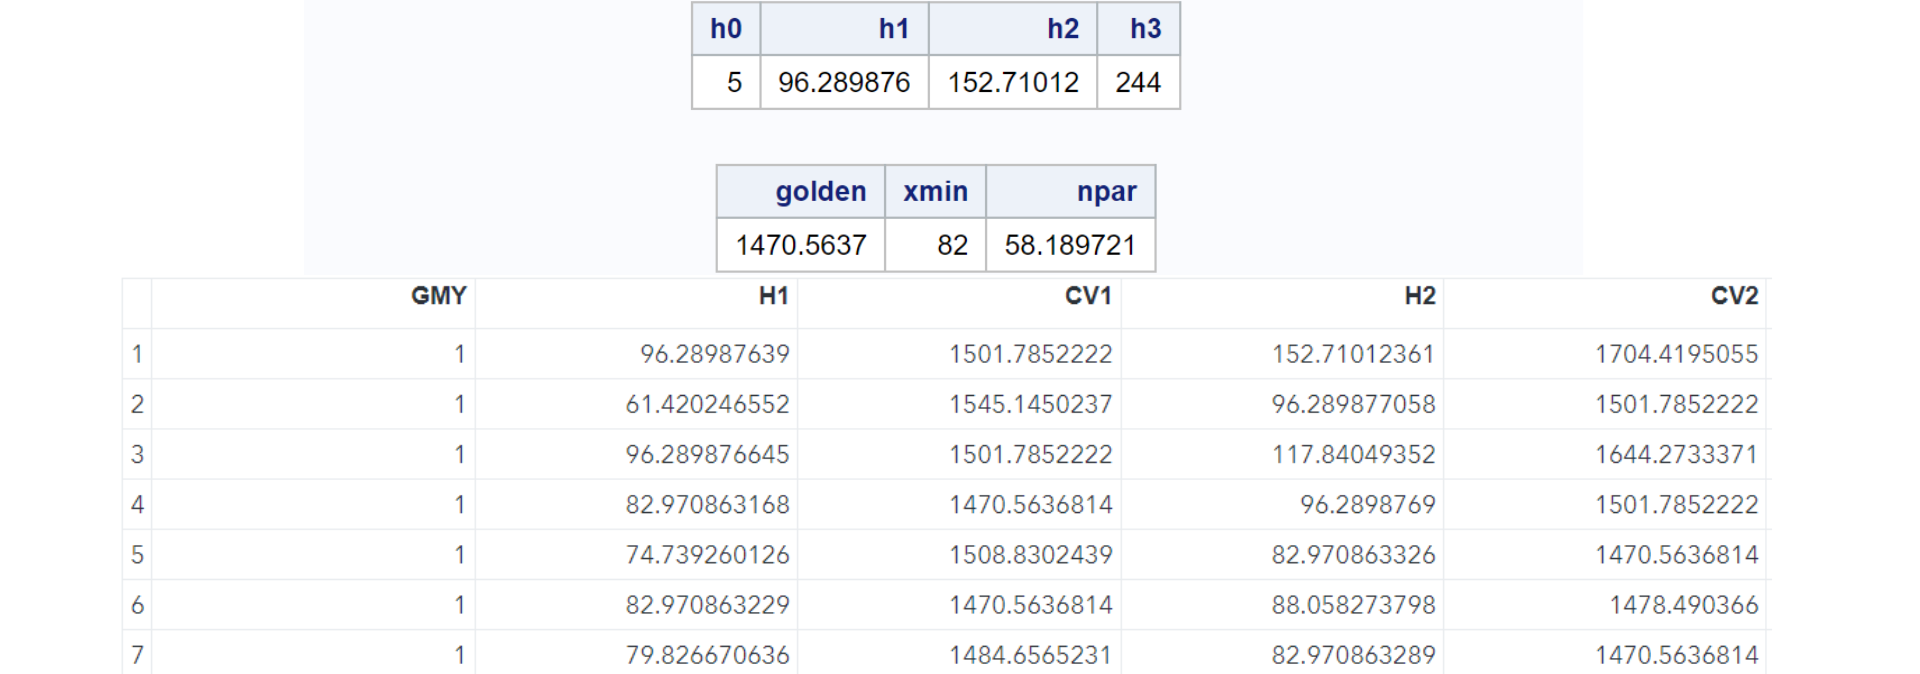
\includegraphics[width=1.0\textwidth]{golden_sas.png}
    \caption{Saída da função \texttt{Golden} no SAS.}
\label{fig:golden_sas}
\end{figure}

\begin{figure}[H]
    \centering
    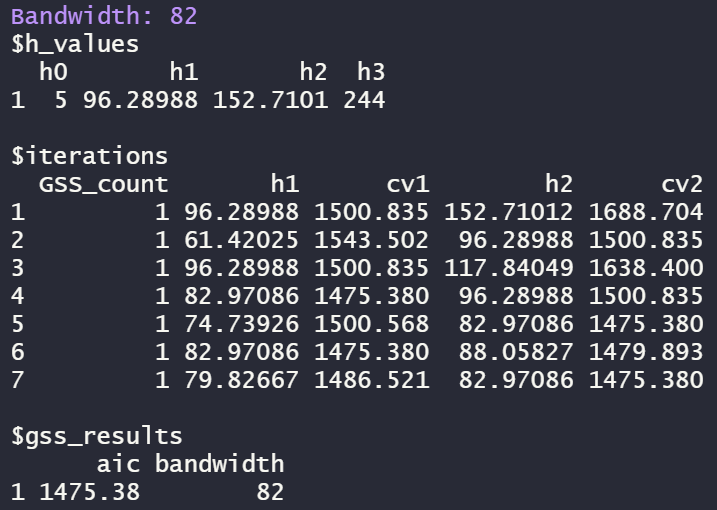
\includegraphics{golden_R.PNG}
    \caption{Saída da função \texttt{Golden} no \texttt{R}.}
\label{fig:golden_R}
\end{figure}

Os resultados do \texttt{R} foram equivalentes aos obtidos usando a macro original do SAS. Foram necessárias sete iterações para se obter o valor ideal para o parâmetro de suavização. Como \texttt{globalmin} recebeu \texttt{FALSE} como argumento, o algoritmo da \textit{Golden Section Search} é executado apenas uma vez (\texttt{GSS\_count=1}), partindo do intervalo inicial $(h_0; h_3)=(5; 244)$. O valor ótimo encontrado para o \textit{bandwidth} foi de 82, pois resulta no mínimo de 1476,69 para a estatística AIC. Em geral, os valores do AIC não são idênticos aos do SAS (resultado final de 1470,56), por questões de arredondamento nas iterações, mas isso não compromete a convergência do algoritmo, nem o \textit{bandwidth} encontrado.

Além do exemplo apresentado, foram executados diversos outros testes para verificar o funcionamento adequado do código no \texttt{R}, sempre comparando-se aos valores obtidos no SAS. Para a função \texttt{Golden}, alguns desses resultados estão resumidos na Tabela \ref{resultados_golden}.

\begin{table}[htb]
\caption{Valores encontados pela função \texttt{Golden} para o parâmetro de suavização, por modelo, método e critério.}
\centering
\begin{tabular}{l|r|r|r|r|r}
\hline
\multicolumn{2}{c|}{\multirow{2}{*}{Modelo}} & \multicolumn{2}{c|}{Fixo} & \multicolumn{2}{c}{Adaptável} \\
\cline{3-6}
\multicolumn{2}{l|}{} & CV & AIC & CV & AIC\\
\hline
\multicolumn{2}{c|}{BNIZ} & 199,96 & 199,96  & 230 &  82    \\
\multicolumn{2}{c|}{PIZ} & 733,70 & 36,98  & 230 &  56    \\
\multicolumn{2}{c|}{Binomial Negativa} & 189,74 & 156,67 & 230 &  82  \\
\multicolumn{2}{c|}{Poisson} & 733,70 & 47,21 & 48 &  79   \\
            \hline
\end{tabular}
\label{resultados_golden}
\end{table}

Olhando apenas para os valores de \textit{bandwidth} encontrados, não se pode concluir sobre o melhor modelo a ser utilizado. No entanto, a partir desses diferentes resultados, pode-se testar a execução da \texttt{gwzinbr} e tirar a conclusão a partir das medidas de ajustamento.

Em geral, o \textit{bandwidth} adaptável é mais versátil do que o fixo, pois funciona bem mesmo quando há diferenças na densidade dos dados ao longo das localizações, conforme descrito na Seção \ref{secao_3_2}. Quanto ao critério de minimização, o AIC é interessante por servir como medida comparativa entre modelos. E, por fim, a distribuição BNIZ pode ser usada como ponto de partida com o argumento \texttt{force = FALSE}, de forma que o algoritmo acomode a distribuição aos dados.

Ao se comparar o ajuste dos diferentes modelos possíveis, os melhores resultados foram os das distribuições binomial negativa e binomial negativa inflacionada de zeros, com parâmetro de suavização igual a 82 \citep{dasilva2023}, encontrado para o método adaptável com critério AIC, conforme a Tabela \ref{resultados_golden}.

\section{gwzinbr}

%Nesta subseção, a análise segue como um estudo de caso dos dados reais da COVID-19.

%O objetivo principal desta seção consiste em verificar e comparar as diferenças que existem no modelo que já foi apresentado em \cite{dasilva2023}, em que foi utilizada a macro GWZINBR implementada em SAS, com os resultados obtidos através da função \texttt{gwzinbr} no \texttt{R}. Em ambos, foi utilizada a distribuição binomial negativa inflacionada de zeros.

Tendo selecionado o valor para o parâmetro de suavização, o próximo passo é o ajuste do modelo através da função \texttt{gwzinbr}:

\begin{lstlisting}[language=R]
> gwzinbr(data = korea_base_artigo,formula = n_covid1~Morbidity+
high_sch_p+ Healthcare_access+diff_sd+Crowding+Migration+
Health_behavior, xvarinf = c("Healthcare_access", "Crowding"), 
long = "x", lat = "y", offset = "ln_total",
method = "adaptive_bsq",  model = "zinb", distancekm = TRUE,
h= 82, force = TRUE)
\end{lstlisting}  

Algumas das saídas resultantes são apresentadas nas Figuras \ref{fig:rbniz_gof_sas} até \ref{fig:global_R}, alternando os \textit{outputs} do SAS e do \texttt{R}.

\begin{figure}[!htb]
    \centering
    \includegraphics[width=0.9\textwidth]{rbniz_gof_sas.png}
    \caption{Medidas de ajustamento e medidas resumo das estimativas dos parâmetros do modelo RBNIZGP no SAS.}
\label{fig:rbniz_gof_sas}
\end{figure}

%\begin{figure}[!htb]
%    \centering
%    \includegraphics[width=0.9\linewidth,height=0.55\linewidth]{rbniz_gof_r.PNG}
%    \caption{Medidas de ajustamento e medidas resumo das estimativas dos parâmetros do modelo RBNIZGP no \texttt{R}.}
%\label{fig:rbniz_gof_r}
%\end{figure}

\begin{figure}[!htb]
    \centering
    \includegraphics[width=0.9\textwidth]{rbniz_gof_r.PNG}
    \caption{Medidas de ajustamento e medidas resumo das estimativas dos parâmetros do modelo RBNIZGP no \texttt{R}.}
\label{fig:rbniz_gof_r}
\end{figure}

%\newpage

As diferenças que aparecem nos resultados do \texttt{R} (Figura \ref{fig:rbniz_gof_r}), em relação aos do SAS (Figura \ref{fig:rbniz_gof_sas}), estão, em sua maioria, presentes apenas nas casas decimais. Conforme explicado na Seção \ref{secao_5_2}, isso ocorre por causa de diferenças intrínsecas dos dois \textit{softwares}, mas não compromete a interpretação dos resultados e as conclusões retiradas. O mesmo vale para os demais resultados apresentados nesta Seção.

A primeira mensagem (\textit{NOTE}) presente nas Figuras \ref{fig:rbniz_gof_sas} e \ref{fig:rbniz_gof_r} afirma que o número de zeros existentes na variável resposta é menor do que a quantidade de zeros esperada, indicando que não há necessidade de se usar um modelo inflacionado de zeros. De acordo com \cite{dasilva2023}, a distribuição binomial negativa tem um bom ajuste e seria suficiente para representar esses dados. No entanto, optou-se por apresentar os resultados da BNIZ neste trabalho, pois com ela ganha-se informações adicionais acerca do elevado número de zeros em algumas localidades.

Em geral, o modelo apresentado teve um bom ajuste, com medidas de pseudo-$R^2$ próximas de 1 (\texttt{pct\_ll} e \texttt{adj\_pct\_ll}). Em relação às estimativas dos parâmetros, seus 244 valores locais podem ser acessados na saída da função, mas apenas alguns quantis e algumas estatísticas descritivas são apresentadas nas Figuras \ref{fig:rbniz_gof_sas} e \ref{fig:rbniz_gof_r}, para se ter uma visão geral desses resultados.

Pode-se observar que para os parâmetros \textit{high\_sch\_p}, \textit{Healthcare\_access} e \textit{Migration}, os valores estimados são principalmente negativos, indicando que o aumento na proporção de pessoas com 2° grau completo, no acesso à saúde e na migração são aspectos que costumam estar associados a uma diminuição nos casos de COVID-19. Já as covariáveis referentes a comorbidades, dificuldade no distânciamento social, aglomeração e comportamento da saúde costumam ter uma relação positiva com a quantidade de casos.

Vale mencionar que para todas as covariáveis, as estimativas dos parâmetros têm valores mínimos negativos e valores máximos positivos, ressaltando a importância de se trabalhar com modelos locais para se observar as diferenças nas relações entre essas variáveis e a resposta em diferentes regiões. As significâncias locais dessas associações podem ser acessadas juntamente com as estimativas completas. %Já o teste mais geral de significância do modelo é mostrado nas Figuras \ref{fig:rbniz_gof_r} e \ref{fig:rbniz_gof_sas} e resultou em um p-valor de 0,0089, indicando que o modelo é relevante para explicar o comportamento da variável resposta.

%**conferir com o Alan sobre esse teste t geral e sobre o nome das medidas.

%\newpage
%comentei agora

\begin{figure}[!htb]
    \centering
    \includegraphics[width=0.9\textwidth]{se_sas.png}
    \caption{Quantis e estatísticas descritivas para os erros padrão das estimativas dos parâmetros do modelo RBNIZGP no SAS.}
\label{fig:se_sas}
\end{figure}

\begin{figure}[!htb]
    \centering
    \includegraphics[width=0.9\textwidth]{se_R.png}
    \caption{Quantis e estatísticas descritivas para os erros padrão das estimativas dos parâmetros do modelo RBNIZGP no \texttt{R}.}
\label{fig:se_R}
\end{figure}

Observando as médias dos erros padrão nas Figuras \ref{fig:se_sas} e \ref{fig:se_R}, é possível perceber que os valores são muito similares entre os dois \textit{softwares}, mas que o \texttt{R} resultou em valores um pouco menores. Como exemplos, tem-se uma média de 2,86 para os erros padrão do intercepto no SAS e de 2,67 no \texttt{R}; para a variável \textit{Crowding} esse valor foi de 0,19 no SAS e 0,18 no R; e para o parâmetro de superdispersão \texttt{alpha} os valores médios obtidos foram de 0,34 e 0,28 para o SAS e o \texttt{R}, respectivamente.

%\newpage
%comentei agora

\begin{figure}[!htb]
    \centering
    \includegraphics[width=0.4\textwidth]{zero_infl_part_sas.png}
    \caption{Medidas para as estimativas dos parâmetros inflacionados de zero para o modelo RBNIZGP no SAS.}
\label{fig:zero_infl_part_sas}
\end{figure}

\begin{figure}[!htb]
    \centering
    \includegraphics[width=0.5\textwidth]{zero_infl_part_R.PNG}
    \caption{Medidas para as estimativas dos parâmetros inflacionados de zero para o modelo RBNIZGP no \texttt{R}.}
\label{fig:zero_infl_part_R}
\end{figure}

Uma das partes mais computacionalmente complexas do algoritmo é a do cálculo das estimativas dos parâmetros inflacionados de zeros. Por esse motivo, esses valores estimados e os respectivos erros padrão sofreram algumas diferenças em seus resultados do \texttt{R} quando comparados ao SAS. Além disso, como essas medidas são apresentadas de forma resumida por meio de quantis e estatísticas descritivas, é importante comentar que as funções de cálculo de quantis são estruturalmente diferentes no SAS e no \texttt{R} e costumam resultar em valores diferentes mesmo para cálculos mais diretos e em dados reduzidos.

Tomando o intercepto como exemplo, os quantis das estimativas foram bastante próximos nos dois programas, sendo a maior diferença entre os valores do primeiro quartil, que difere em 6 unidades, conforme as Figuras \ref{fig:zero_infl_part_sas} e \ref{fig:zero_infl_part_R}. Os valores mínimo e máximo coincidem nas duas saídas, enquanto a média apresenta uma grande diferença (-503,00 no SAS e -1732,58 no \texttt{R}) devido a alguns valores extremos que aparecem como consequência das características dos \textit{softwares} explicadas na Seção \ref{secao_5_2}.

Já para as duas variáveis explicativas da parte inflacionada de zeros (\textit{Heathcare\_acces} e \textit{Crowding}), as medidas resumo são muito similares no SAS e no \texttt{R}, existindo diferenças apenas na parte decimal dos valores. O teste de significância dos parâmetros também apresentou resultados equivalentes nos dois \textit{softwares}.

Ainda nas Figuras \ref{fig:zero_infl_part_sas} e \ref{fig:zero_infl_part_R}, os valores dos quartis para as estimativas do parâmetro \textit{Crowding} são maiores do que os respectivos resultados para \textit{Healthcare\_access}, indicando que a associação entre o nível de aglomeração e a probabilidade de se ter COVID-19 é mais forte do que a associação entre o acesso à saúde e a probabilidade de se ter essa doença. Essa observação está de acordo com o que foi concluído por \cite{sousa2022}, por meio de testes de significância.

\begin{figure}[!htb]
    \centering
    \includegraphics[width=0.5\textwidth]{se_infl_sas.png}
    \caption{Quantis e estatísticas descritivas para os erros padrão das estimativas dos parâmetros inflacionados de zero do modelo RBNIZGP no SAS.}
\label{fig:se_infl_sas}
\end{figure}

\begin{figure}[!htb]
    \centering
    \includegraphics[width=0.5\textwidth]{se_infl_R.png}
    \caption{Quantis e estatísticas descritivas para os erros padrão das estimativas dos parâmetros inflacionados de zero do modelo RBNIZGP no \texttt{R}.}
\label{fig:se_infl_R}
\end{figure}

Pelas Figuras \ref{fig:se_infl_sas} e \ref{fig:se_infl_R}, é possível notar que os erros padrão da parte inflacionada de zeros foram, em geral, maiores no \texttt{R}. Comparando do SAS para o \texttt{R}, respectivamente, as médias do intercepto foram de magnitude $10^{19}$ e $10^{20}$, as do parâmetro \textit{Crowding} foram da magnitude de $10^{18}$ e $10^{19}$ e as de \textit{Healthcare\_access} tiveram a mesma magnitude de $10^{18}$, mas com maior valor no \texttt{R} ($2,42<7,73$).

\begin{figure}[!htb]
    \centering
    \includegraphics[width=0.6\textwidth]{global_sas.png}
    \caption{Estimativas dos parâmetros e medidas de ajustamento para a versão global do modelo RBNIZGP no SAS.}
\label{fig:global_sas}
\end{figure}


\begin{figure}[!htb]
    \centering
    \includegraphics[width=0.6\textwidth]{global_R.png}
    \caption{Estimativas dos parâmetros e medidas de ajustamento para a versão global do modelo RBNIZGP no SAS.}
\label{fig:global_R}
\end{figure}

As saídas para o modelo global, nas Figuras \ref{fig:global_sas} e \ref{fig:global_R}, foram idênticas entre SAS e \texttt{R}, considerando as casas decimais disponíveis para visualização. Além disso, as estimativas dos parâmetros condizem com a distribuição geral de estimativas apresentada anteriormente para os modelos locais: intercepto negativo; parâmetro de superdispersão próximo de 3; comorbidade, dificuldade de distanciamento social, aglomeração e comportamento da saúde sendo aspectos que se relacionam de forma positiva com o número de casos de COVID-19; enquanto proporção de pessoas com ensino médio completo, nível de acesso à saúde e migração possuem correlação negativa com a resposta.

A parte inflacionada de zeros também resultou em valores positivos para as estimativas dos parâmetros \textit{Healthcare\_access} e \textit{Crowding}, indicado que o aumento nessas variáveis é acompanhado de aumento na probabilidade de se ter COVID-19, estando de acordo com o que foi observado nos modelos locais. Além disso, os erros padrão não apresentaram valores muito elevados, e os testes $t$ para todas as covariáveis resultaram em $p$-valores pequenos, representando a significância dos parâmetros na explicação sobre a quantidade de casos da doença.

Em geral, as medidas de ajustamento indicam que o modelo global teve ajuste inferior ao RBNIZGP. Os indicadores de pseudo-$R^2$ que eram próximos de 1 para o modelo mencionado, estão entre 0,3 e 0,4 para a versão global. Ademais, tanto o AIC como o AICc aumentaram quando comparados aos seus valores no modelo RBNIZGP ($1420,44<1520,59$ e $1472,83<1521,94$).

%\newpage

\section{Visualização dos Resultados}

Após o ajuste do modelo RBNIZGP através da função \texttt{gwzinbr}, é interessante observar como as variáveis envolvidas e as estimativas do modelo se distribuem espacialmente ao longo do país. Para isso, foram construídos mapas no \texttt{R} através do pacote \href{https://cran.r-project.org/web/packages/leaflet/index.html}{leaflet}, com versões interativas disponíveis no \href{https://rpubs.com/julianamrosa/1198864}{RPubs}. Entre as covariáveis utilizadas no ajuste, a variável de aglomeração, \textit{Crowding}, foi escolhida para exemplificar essas distribuições espaciais, por ser de grande relevância para a explicação do fenômeno e por estar incluída tanto na parte inflacionada de zeros como na parte não inflacionada do modelo.

\begin{figure}[!htb]
    \centering
    \includegraphics[width=0.8\textwidth]{mapa resposta.png}
    \caption{Distribuição espacial do número de casos de COVID-19 na Coreia do Sul durante fase inicial da pandemia}
\label{fig:mapa resposta}
\end{figure}

A Figura \ref{fig:mapa resposta} apresenta a distribuição espacial dos casos de COVID-19 pela Coreia do Sul na fase inicial da pandemia, em que se observa uma maior concentração de zeros. Isso reforça a ideia de um comportamento inflacionado de zeros e que, complementado com a superdispersão identificada nos dados (os valores de casos de COVID-19 podem chegar até o máximo de 4155), caracteriza uma provável distribuição binomial negativa inflacionada de zeros. 

É interessante observar que as regiões com maiores números de casos são também aquelas que figuram entre as principais do país: Seul (capital), Busan (onde está localizado o porto mais movimentado do país) e Daejeon (polo tecnológico). As localizações dessas cidades podem ser identificadas na Figura \ref{fig:mapa Coreia do Sul}. 


\begin{figure}[!htb]
    \centering
    \includegraphics[width=0.8\textwidth]{mapa coreia do sul.png}
    \caption{Mapa da Coreia do Sul}
    \caption*{\footnotesize Fonte: Google Maps, com adaptações}
\label{fig:mapa Coreia do Sul}
\end{figure}

\begin{figure}[!htb]
    \centering
    \includegraphics[width=0.8\textwidth]{mapa_explicativa.png}
    \caption{Distribuição espacial do nível de aglomeração (\textit{Crowding}) na Coreia do Sul}
\label{fig:mapa_explicativa}
\end{figure}

%\newpage

Já na Figura \ref{fig:mapa_explicativa} observa-se o comportamento espacial do nível de aglomeração (variável explicativa \textit{Crowding}). São níveis que variam de moderado a baixo, e que traduzem uma política local ostensiva de combate à doença desde a fase inicial da pandemia.\footnote{BBC. Coronavírus: o que está por trás do sucesso da Coreia do Sul para salvar vidas em meio à pandemia. Disponível em: \url{https://www.bbc.com/portuguese/internacional-51877262}. Acesso em: 02 de junho de 2024}

\begin{figure}[!htb]
    \centering
    \includegraphics[width=0.8\textwidth]{mapa_beta.png}
    \caption{Distribuição espacial das estimativas do parâmetro \textit{Crowding} no modelo RBNIZGP na Coreia do Sul}
\label{fig:mapa_beta}
\end{figure}

As estimativas para o parâmetro \textit{Crowding} e suas distribuições no espaço podem ser conferidas na Figura \ref{fig:mapa_beta}. A visualização auxilia no entendimento inicial de como essa variável pode impactar o número de contaminações pela doença. As cores mais claras no mapa representam valores mais próximos de zero, sugerindo que a aglomeração não tenha uma associação tão forte com a quantidade de casos naquelas regiões.

Uma pequena porção da região litorânea do país (em tons escuros de vermelho) indica uma associação negativa com a resposta, ou seja, o aumento no nível de aglomeração é acompanhado de um decréscimo no número de casos nesses locais. Em sentido contrário, porções em tons de azul mais escuro, localizadas principalmente próximo da capital, sugerem uma correlação positiva.

%\newpage

\begin{figure}[!htb]
    \centering
    \includegraphics[width=0.8\textwidth]{mapa_lambda.png}
    \caption{Distribuição espacial das estimativas do parâmetro \textit{Crowding} inflacionado de zeros no modelo RBNIZGP na Coreia do Sul}
\label{fig:mapa_lambda}
\end{figure}

A Figura \ref{fig:mapa_lambda} apresenta as estimativas calculadas para o parâmetro \textit{Crowding} na parte inflacionada de zeros do modelo. Ou seja, os valores dos coeficientes, nesse caso, representam a relação entre o nível de aglomeração e a ocorrência ou não de COVID-19. Assim, observa-se que a região mais nordeste do mapa contém alguns valores negativos para representar essa relação. Porém, de forma geral, na maior parte do país a aglomeração é uma característica que está associada positivamente com a probabilidade de se ter a doença.

Além disso, alguns locais próximos a Seul apresentaram valores nulos para a estimativa do coeficiente inflacionado de zeros, indicando que a aglomeração não têm significância na explicação da ocorrência de COVID-19 nessas localizações. E o único local onde o valor estimado foi muito elevado foi no condado de Hapcheon, mais ao sul do país, representado em azul escuro.

\begin{figure}[!htb]
    \centering
    \includegraphics[width=0.8\textwidth]{mapa_alpha.png}
    \caption{Distribuição espacial das estimativas do parâmetro de superdispersão no modelo RBNIZGP na Coreia do Sul}
\label{fig:mapa_alpha}
\end{figure}

Por fim, a Figura \ref{fig:mapa_alpha} mostra a distribuição espacial das estimativas para o parâmetro de superdispersão $\alpha$. A partir desse mapa, é possível ter uma ideia inicial de quais distribuições são mais adequadas para representar os dados de resposta em localidades específicas. Valores maiores para o parâmetro sugerem que distribuições que acomodam esse comportamento de alta variabilidade (como a binomial negativa e a binomial negativa inflacionada de zeros) são as mais indicadas para a modelagem. Isso ocorre para o leste do país, enquanto que para o oeste distribuições como a Poisson ou a Poisson inflacionada de zeros seriam o suficiente para descrever o número de casos. 

\chapter{Conclusões}

O presente trabalho alcançou seu objetivo principal ao implementar um pacote \texttt{R} (atualmente já publicado no CRAN) para o algoritmo de Regressão Binomial Negativa Inflacionada de Zeros Geograficamente Ponderada (RBNIZGP), proposto por \cite{dasilva2023} e previamente implementado em SAS pelos referidos autores. O pacote \texttt{gwzinbr}, ainda que focado na RBNIZGP, é capaz de ajustar espacialmente dados de contagem que apresentem comportamentos compatíveis com pelo menos outras três distribuições conhecidas (Poisson, Binomial Negativa e Poisson Inflacionada de Zeros). 

A comparação dos resultados obtidos por ambos os \textit{softwares} a partir de um estudo de caso realizado pelos autores da teoria possibilitou não somente a compreensão do método pelas realizadoras deste relatório, como também a experiência de desenvolvimento e gerenciamento de pacotes no \texttt{R} e um maior entendimento sobre o SAS e seus aspectos computacionais. Ainda que algumas saídas não tenham resultado em uma replicação exata, o pacote desenvolvido em \texttt{R} se mostrou capaz de alcançar os resultados esperados, sendo uma alternativa acessível para pesquisadores.

Como as diferenças nos tempos de execução entre SAS e \texttt{R} mostraram que o pacote \texttt{gwzinbr} ainda pode ser melhorado em termos de eficiência computacional, espera-se que contribuições futuras possam otimizar o código. Uma sugestão seria o uso de processamento pararelo, o qual permite o aproveitamento de recursos computacionais físicos para que diferentes núcleos de uma máquina possam realizar diferentes cálculos ao mesmo tempo. Também é interessante a aplicação futura desse algoritmo em novos conjuntos de dados e a realização de estudos de simulação para melhor comparação entre as funções em SAS e \texttt{R}.

%Métodos alternativos também podem ser buscados para minimizar o uso de loops e aproveitar as estruturas e operações de matrizes.

\addcontentsline{toc}{section}{\textbf{Referências}}
%\bibliographystyle{abntex2-alf}
\bibliographystyle{bbs2}
\bibliography{biblio}


\end{document}
